\section{The Setup}
\subsection{Introduction}

As the old adage says, ``a picture is worth a thousand words.'' Statisticians, and scientists in general, rely on graphical displays---pictures, essentially---to communicate information, analysis, and results. We deploy graphical displays to efficiently communicate data set information content to other statisticians, and, perhaps more importantly, to non-statisticians. As technology generates more data, and statistical analysis becomes more widespread, graphical displays become more important; therefore, our graphic-making abilities must improve. The R data visualization package \verb|ggplot2| stands out as the single most downloaded R package, which highlights the importance of graphical displays and the continued need for graphical innovations \citep{rdoc}.

In this chapter we focus on one type of graphical display: heat maps. We argue uniform resolution throughout the heat map domain, the current best practice, inadequately accomodates spatially varying data density; and misses an opportunity to communicate data density information. We offer a solution that addresses this shortcoming.

\subsection{Bernoulli Swings}

% Note the variable \verb|des|, short for `description,' that describes pitch outcomes. In this study, we use swing outcomes described in \verb|des| to define a Bernoulli random variable $S$ (Section 3.1) that equals one for a hit, and equals zero for {\it any} swing that does not result in a hit. 

Baseball centers around a series of contests between the hitter and the pitcher, comprised of pitches the hitter can swing at, or choose not to swing at. We treat every swing as a trial, and success or failure should be evaluated independently from the count in the at bat at the time of the trial. Accordingly, we consider every swing a trial in this study.  This differs from other studies that include only at bat ending pitches \citep{Cross2015}, \citep{Baumer2010}, \citep{Fast2011}. These studies {\it exclude} from analysis swinging strikes that do not end at bats, and foul balls; but {\it include} pitches that end at bats, even if the hitter did not swing. We consider these latter events a possible mistake in the hitter's decision making, not a failed swing attempt. Based on these rationales, in this work we consider every swing a trial, with some probability of success. 

Accordingly, we define success as swings where the variable \verb|des|, short for description, equals \verb|in play, no out|, and failure as swings where \verb|des| equals \verb|Foul|, \verb|Foul (Runner Going)|, \verb|Foul Tip|, \verb|In play out(s)|, \verb|Swinging Strike|, or \\ \verb|Swinging Strike (Blocked)|. With this interpretation of the data, next we explain the setup and interpretation of a baseball strike zone heat map.

\subsection{Empirical Strike Zone Heat Maps}

Empirical baseball strike zone heat maps cover the two-dimensional, vertical face of the strike zone with a grid, containing empirical success probabilities ($\hat{p}$, defined below) in each grid box.  We start with a data set containing PITCHf/x\textsuperscript{\textregistered} data on 1,932 right-handed hitters, taking 1,582,581 swings between 2008 and 2015.  Let $b = 1, \dots, 627$ index grid boxes. Let $i = 1, \dots, 1,582,581$ index swings, and define $n_{b} = \displaystyle\sum_{i} \text{I}_{\{i \in b \}}$ as the total number of swings in box $b$.

Define Bernoulli random variable, $S_{i}$, to equal one for swing success and zero for swing failure, and define $\hat{p}_{b} = \frac{1}{n_{b}} \displaystyle\sum_{i} S_{i} \cdot \text{I}_{\{i \in b \}}$ as the empirical box $b$ success probability. Figure 1 displays the resulting empirical heat map for this data. The graphic maps the empirical hitter success probability, $\hat{p}_{b}$, to a color on a spectrum, for pitches that passed through the space represented by that grid box.
  \begin{figure}[H]
	\centering
	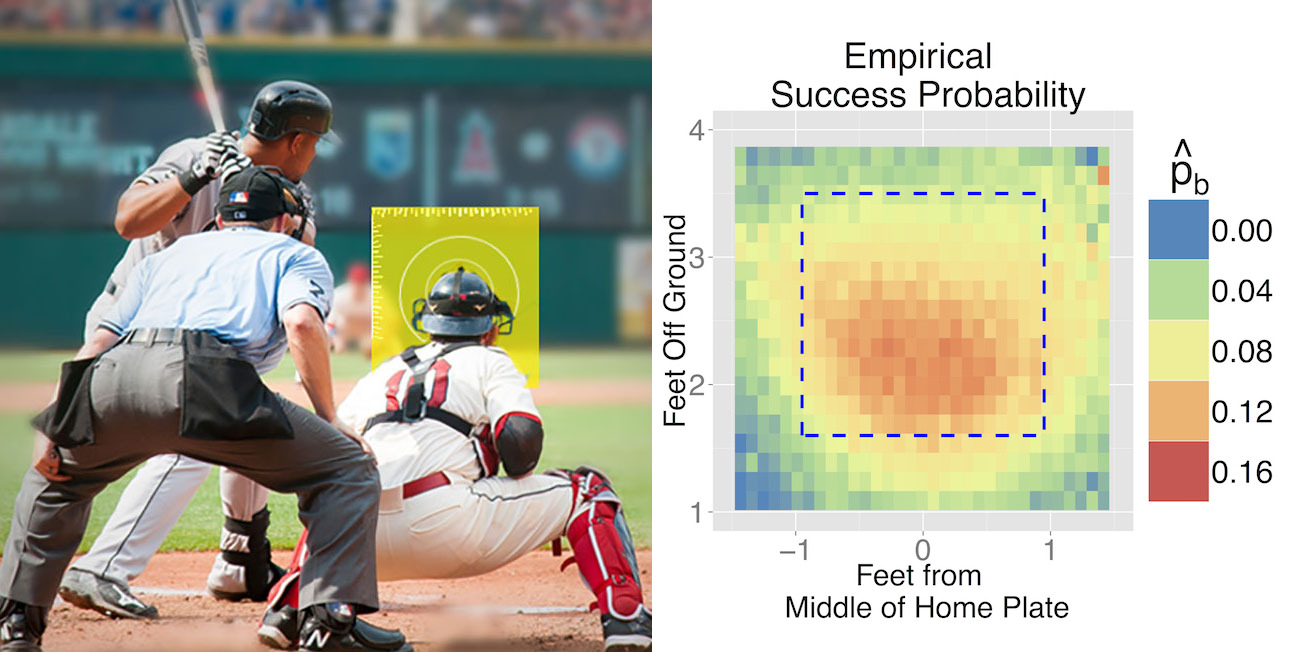
\includegraphics[scale=.35]{Images/SZandMothership.jpg} 
  \caption{The setup, and the heat map. The setup in the image on the left demonstrates the proper perspective for understanding the heat map on the right. This heat map grids the hitting zone with approximately 3/4 inch by 3/4 inch boxes. The dashed blue line on the right outlines, roughly, the yellow box on the left. Each grid box color represents the empirical success probability ($\hat{p}_{b}$) of hitter swings at pitches passing through that box.  The data consists of 1,932 right handed hitters, swinging at 1,582,581 pitches between 2008 and 2015.}
	\end{figure} 
While not sophisticated statistically, the graphic efficiently conveys empirical spatial success probabilities, by mapping the statistic $\hat{p}_{b}$ to the color spectrum. However, note that the statistician---not the data---determines the map's resolution.

\section{Traditional Heat Maps}

\subsection{Resolution} % ============== =============

Though often overlooked, a heat map's creator {\it chooses} a resolution. This choice determines a uniform grid box size for the heat map, which influences heat map quality and appearance markedly. This influence is analagous to the impact of bin width selection on histogram appearance. 

Also, notice that heat maps fail to convey varying spatial data density, i.e. through the strike zone. With no spatial density information, heat maps conceal estimate sample sizes and variances.  As a rule, heat maps do not communicate this information.

The heat map in Figure 1.2 divides the strike zone into relatively small boxes, because the data supports it.
  \begin{figure}[H]
	\centering
	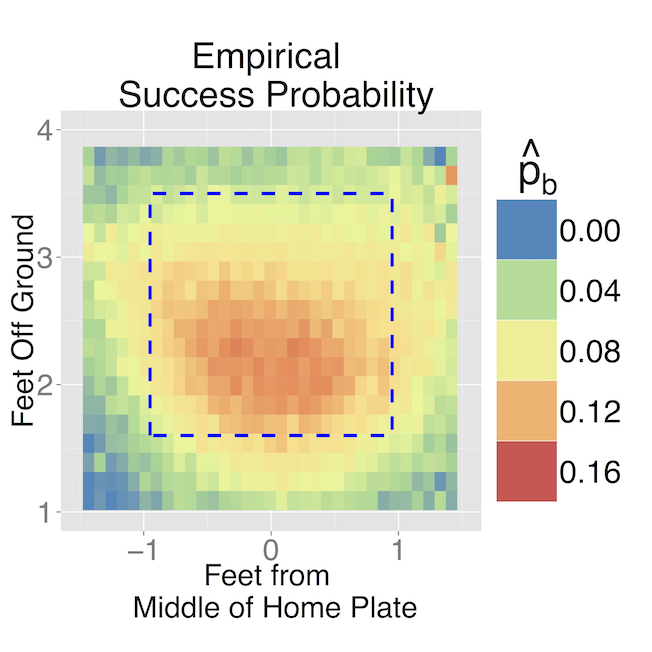
\includegraphics[scale=.4]{Images/Mothership3.jpg} 
  \caption{This heat map grids the hitting zone with approximately 3/4 inch by 3/4 inch boxes. The dashed blue line approximately outlines the strike zone. Each grid box color represents the empirical success probability ($\hat{p}_{b}$) of hitter swings at pitches passing through that box.  The data consists of 1,932 right handed hitters, swinging at 1,582,581 pitches between 2008 and 2015.}
	\end{figure} 
By ``supports it'' we mean the small, spatially specific boxes retain sample sizes large enough to avoid unacceptable $\hat{p}_{b}$ variance inflation. Defining ``acceptable'' variance depends on context and objectives. For example, a pitching coach might want estimates accurate to within 10 batting average points, 95\% of the time. This margin of error, 0.02, requires a sample size of 32 when $p_{b} = 0.09$.\footnote{Note that the variance depends on the mean for a Bernoulli random variable.} In contrast to the data for all right-handed hitters over seven years used for Figure 1.1, individual hitter data sets vary dramatically in size. Hitter data ranges from a single swing to over 10,000 swings. In data sets for individual hitters, then, the resolution choice becomes more complicated. This complexity owes to non-uniform data density, meaning that different regions may support very different resolutions. 

As stated before, the choice of resolution sometimes dramatically affects heat map appearance, but also usefulness. For example, for a heat map overly coarse in regions of interest, the parameter estimates lose value. 

This important resolution decision usually depends on the size and nature of the data set in question, and its spatial dispersion through the domain. In the next section we explore this decision in detail, along with its inherent compromises.

\subsection{Resolution Selection}

In this section, we use batter 425509, a veteran player named Jhonny Peralta, to explore resolution selection and its implications. Our data set includes 9,177 Peralta swings. Peralta's swing data yields the heat map in Figure 1.2, which divides the hitting zone into 16 equally sized boxes. Each box maps $\hat{p}_{b}$ to a color, with box sample sizes, $n_{b}$, printed on box centers. We will use box sample sizes to reference boxes. For example, we will call the box in the lower-left ``box 22.'' (**NOTE: MAKE LABELS BIGGER)
        \begin{figure}[H]
      	\centering
      	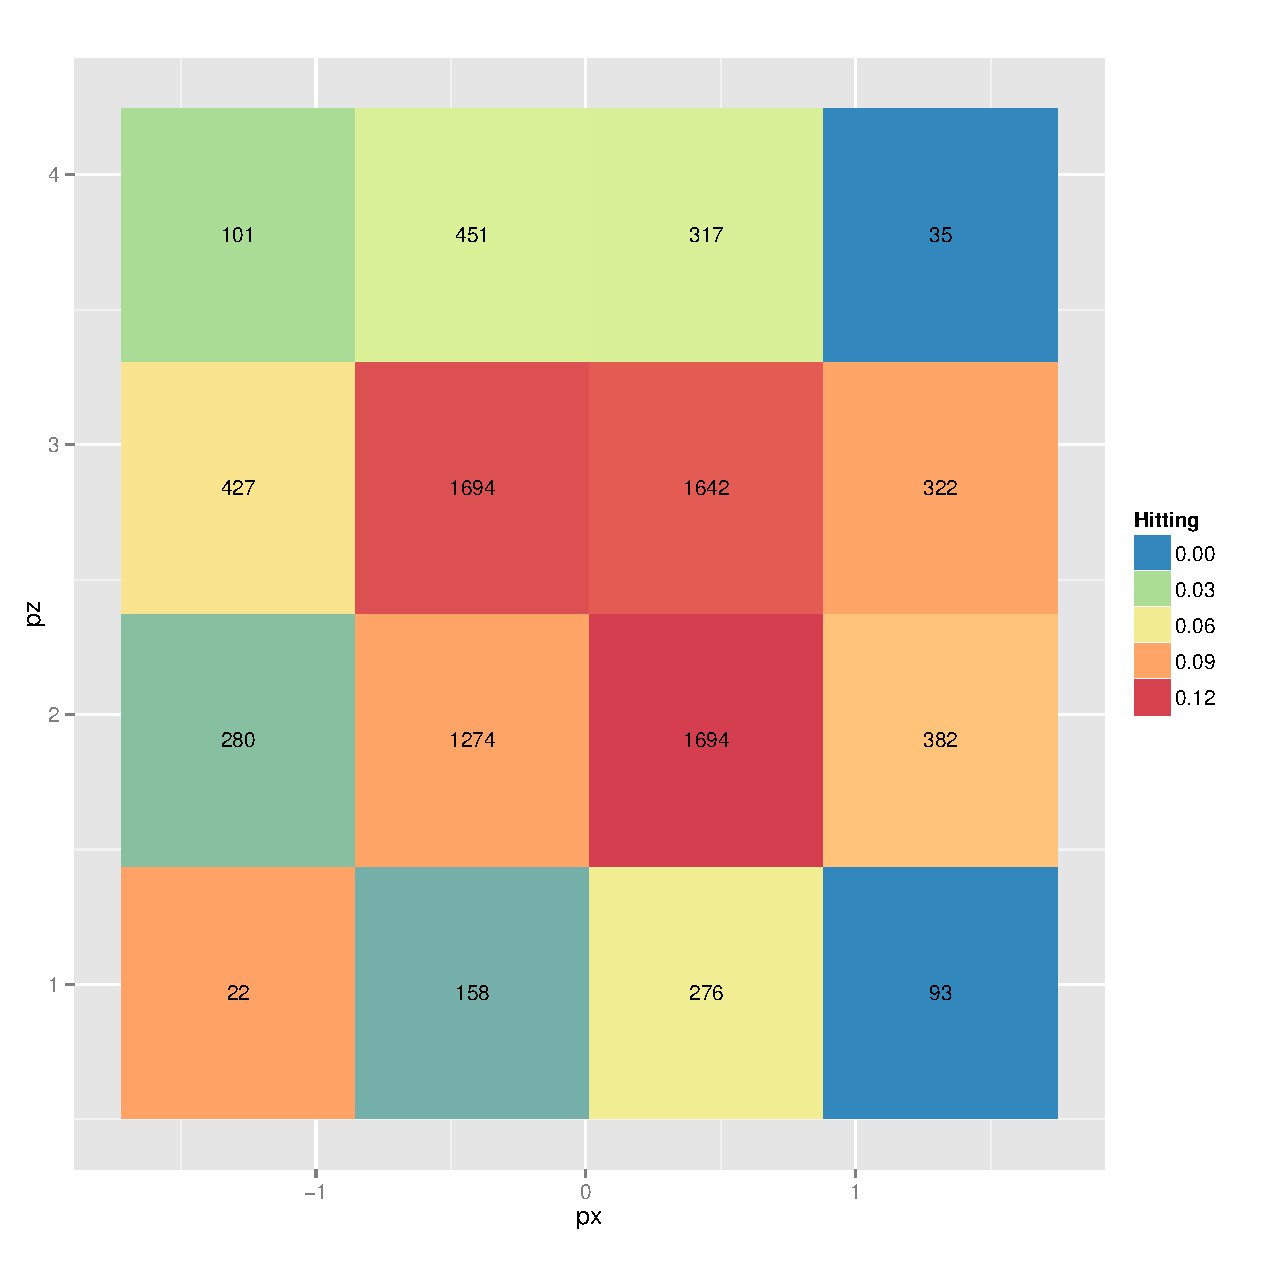
\includegraphics[scale=.35]{Images/Chapter4x4.pdf} 
      	\caption{This four by four heat map shows the empirical batting average of Johnny Peralta, for pitches passing through the space represented by each of 16 square regions of the hitting zone. Each box maps $\hat{p}_{b}$ to a color, with box sample sizes, $n_{b}$, printed on box centers.}
      	\end{figure} 

Notice the four by four resolution suffices for box 22; further subdivision might yield trivially small subdivided-box sample sizes. On the other hand, the center boxes, all with sample sizes above 1200, can and should provide more location specific $\hat{p}$ estimates. This motivates finer resolution in that region of space, but at the expense of box 22. With this trade-off in mind, we subdivide all boxes further. 

For simplicity we divide each box into four equally sized sub-boxes. Note, however, that subdivision algorithms could take countless forms. Figure 3 shows the eight by eight result.
        \begin{figure}[H]
      	\centering
      	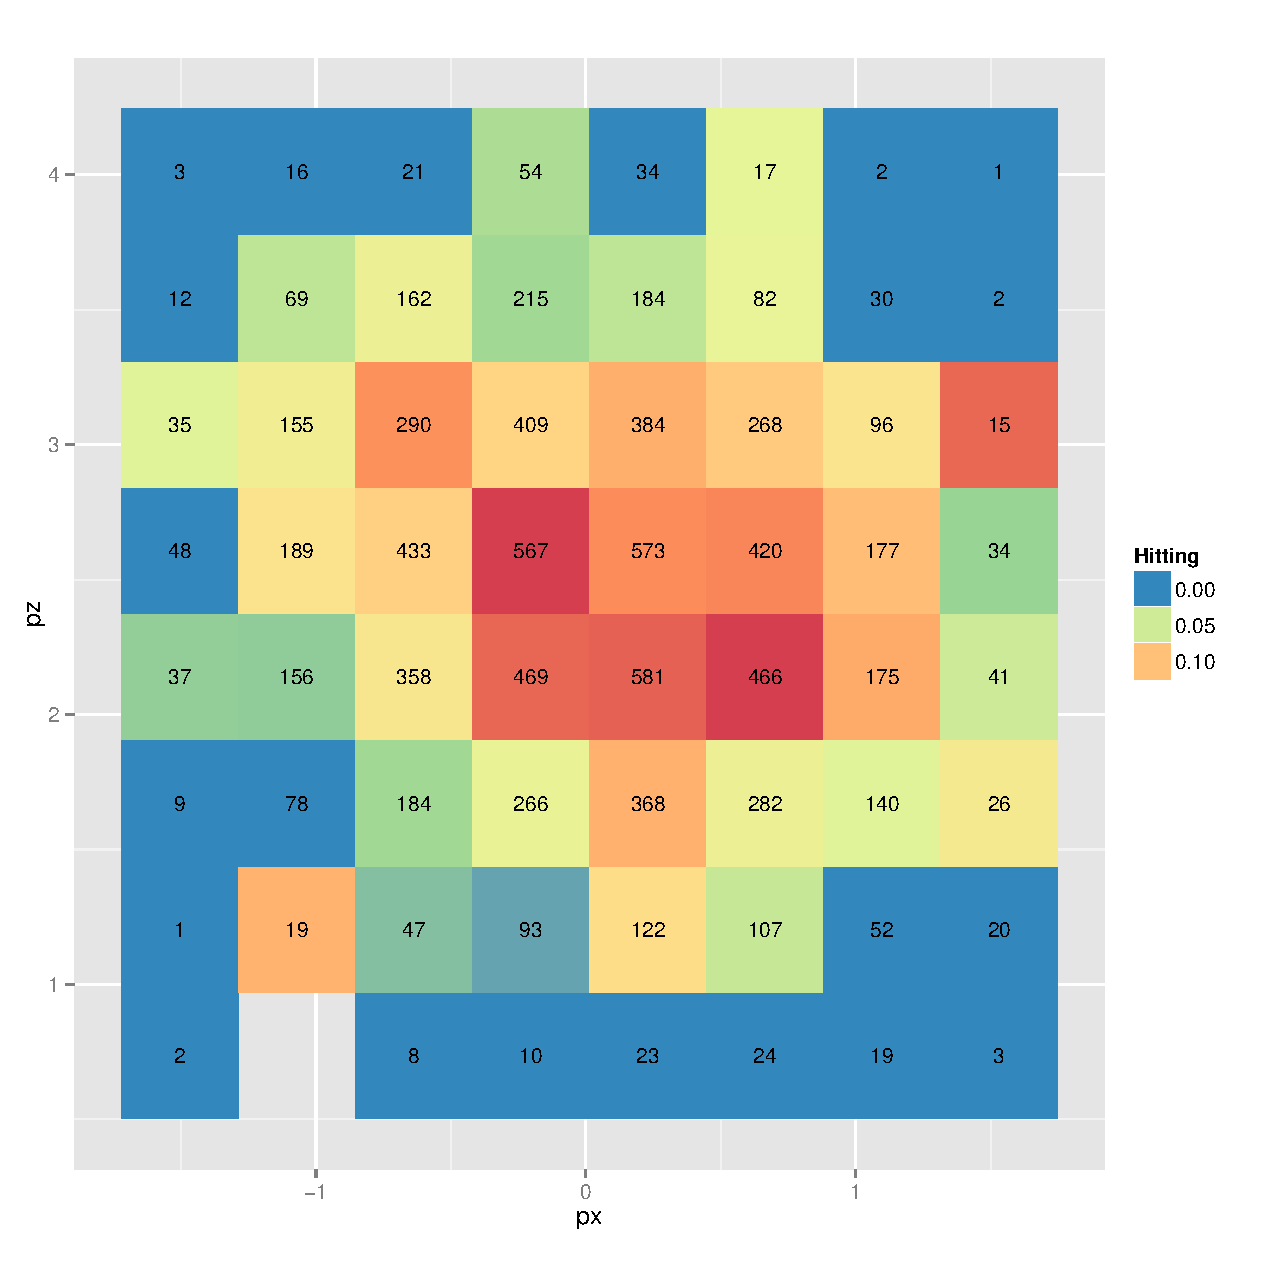
\includegraphics[scale=.25]{Images/Chapter16x16.pdf} 
      	\caption{This eight by eight heat map shows the empirical hitting success probability of Johnny Peralta, for pitches passing through the space represented by each of 64 square regions of the hitting zone. Each box maps $\hat{p}_{b}$ to a color, with box sample sizes, $n_{b}$, printed on box centers. A grey box indicates no pitches passed through that box. Notice that this resolution imparts additional information in the center of the hitting zone, some box sample sizes toward the margin have dropped uninformatively low.}
      	\end{figure} 

The centermost 16 boxes still contain sample sizes sufficient to support low variance $p$ estimates; the minimum of these boxes contains 184 swings. Globally, 24 boxes consist of over 150 swings; and 15 boxes still include more than than 250 swings. These boxes could support further subdivision. On the other hand, many boxes, especially edge boxes, now contain sample sizes generally insufficient to support low variance estimates of $p_{b}$. Twenty-nine boxes contain fewer than 50 swings, and 17 boxes contain fewer than 20 swings. One box recorded zero swings.

With this range of box sample sizes due to the varying spatial density of the data, the heat map at any resolution will contain boxes of exceedingly small sample sizes (high variance), and boxes of unnecessarily large sample size (unnecessarily low variance). Figure 1.4 shows six different resolutions for Peralta's data. We started with one box, and subdivided each box into four at each iteration. This simple resolution increase algorithm plainly illustrates the resolution selection challenge, and provides a foundation for our innovation in the next section. 
        \begin{figure}[H]
      	\centering
      	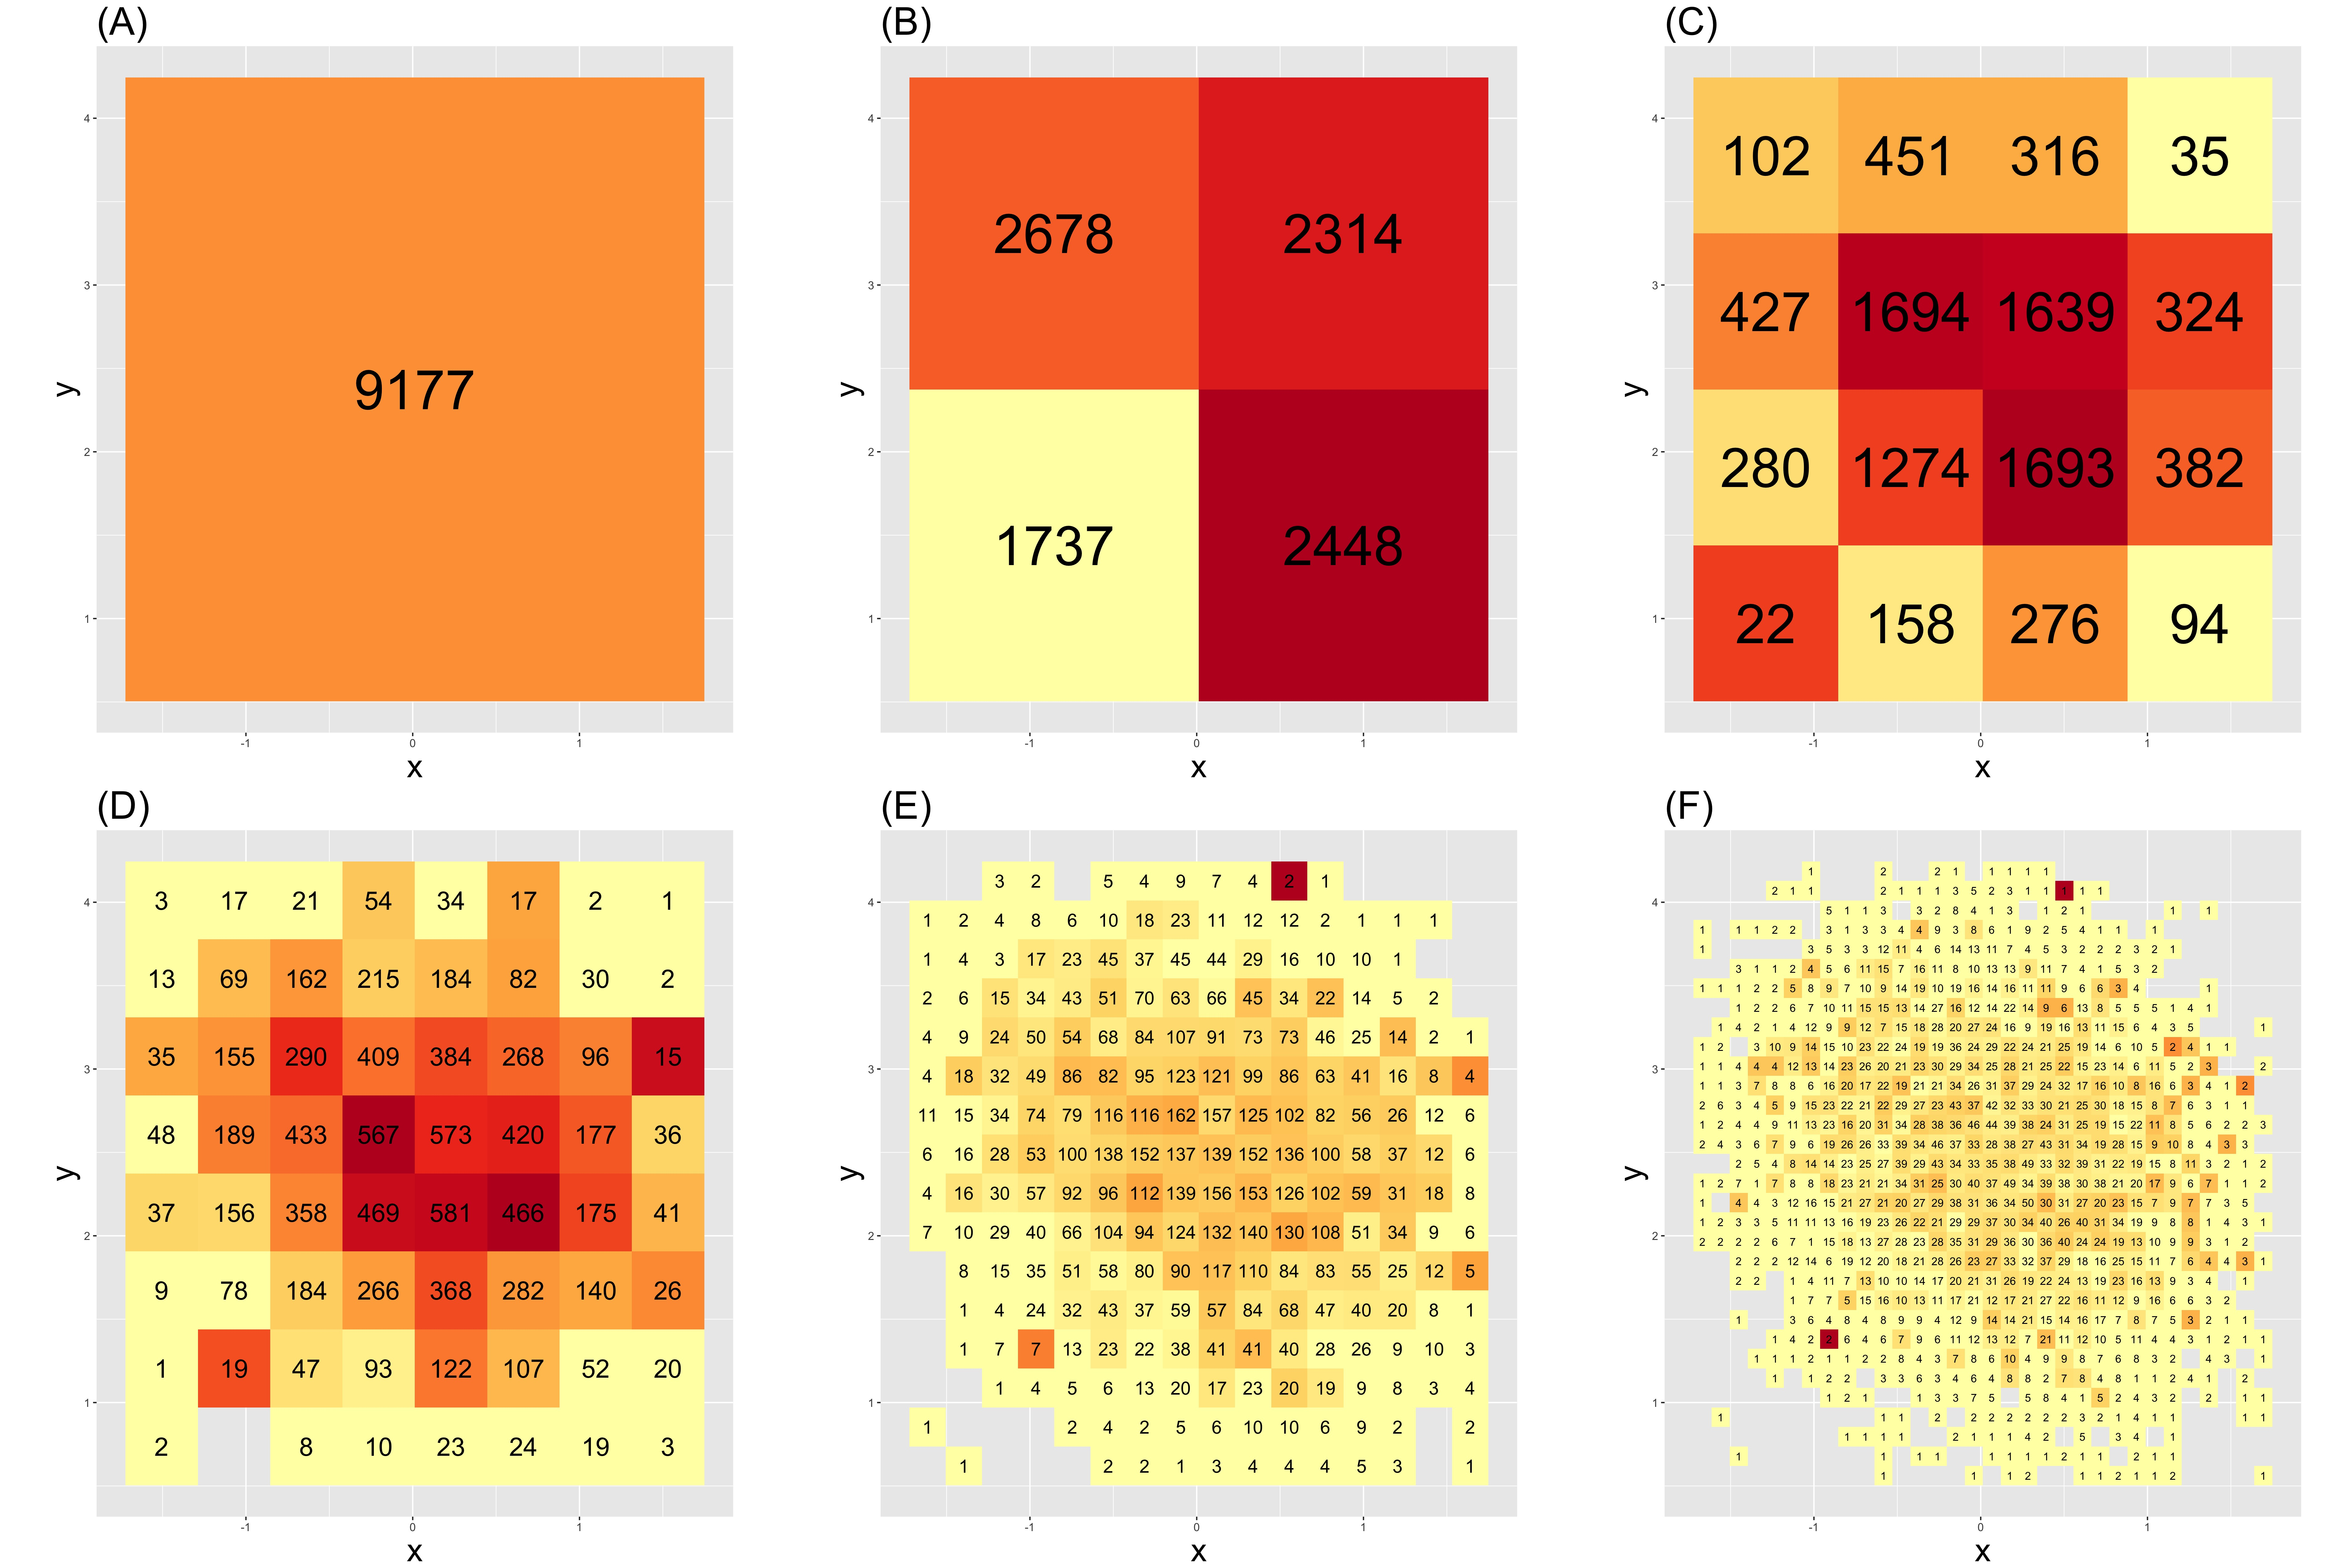
\includegraphics[scale=.055]{Images/Chapter_VarRes.jpg} 
      	\caption{These six heat maps show the same data for Johnny Peralta, at increasing resolutions. The maps range from obviously too coarse to perhaps excessively fine. Notice how dramatically the image changes as the resolution increases. Which resolution yields the highest quality heat map?}
      	\end{figure} 
Which of these five resolutions best balances spatially precise estimates of $p$ with acceptable box sample sizes? The viewer interested in the center of the strike zone might prefer the middle-bottom map, as the box sample sizes support such spatially specific estimates. However, the boxes closer to the edges of the strike zone then contain higher variance, less reliable estimates due to prohibitively small sample sizes. 

All six resolution options include trade-offs. We propose a new heat map approach the eliminates trade-offs. The solution combines multiple resolutions into one map, according to the data's varying spatial density.

\section{Spatially Varying Resolution} % ==========

\subsection{A Solution}

Consider again the heat map in Figure 1.2. Recall box 22 contains 22 swings, a sample size where subdividing would yield uninformatively small sample sizes, and thus prohibitively high estimation variance $\text{Var}(\hat{p}_{b})$. In contrast, box 1694 would support estimates that are more spatially accurate without $\text{Var}(\hat{p}_{b})$ increasing beyond acceptable levels. We propose resolution increase decisions occur box by box, according to an algorithm which includes a stopping rule and a subdivision method. Note that the stopping rule and subdivision algorithm can be defined by the map's creator, offering flexibility to create the heat map structure that suits the data. 

To demonstrate, recall the $16 \times 16$ map in Figure 1.2. On this map we divide all boxes where $n_{b} > 200$, into four smaller, equally sized boxes. Figure 1.5 shows the map before and after the procedure. Moving through all boxes of the map to the left, subdividing when $n_{b} > 200$, yields the heat map to the right.
        \begin{figure}[H]
      	\centering
      	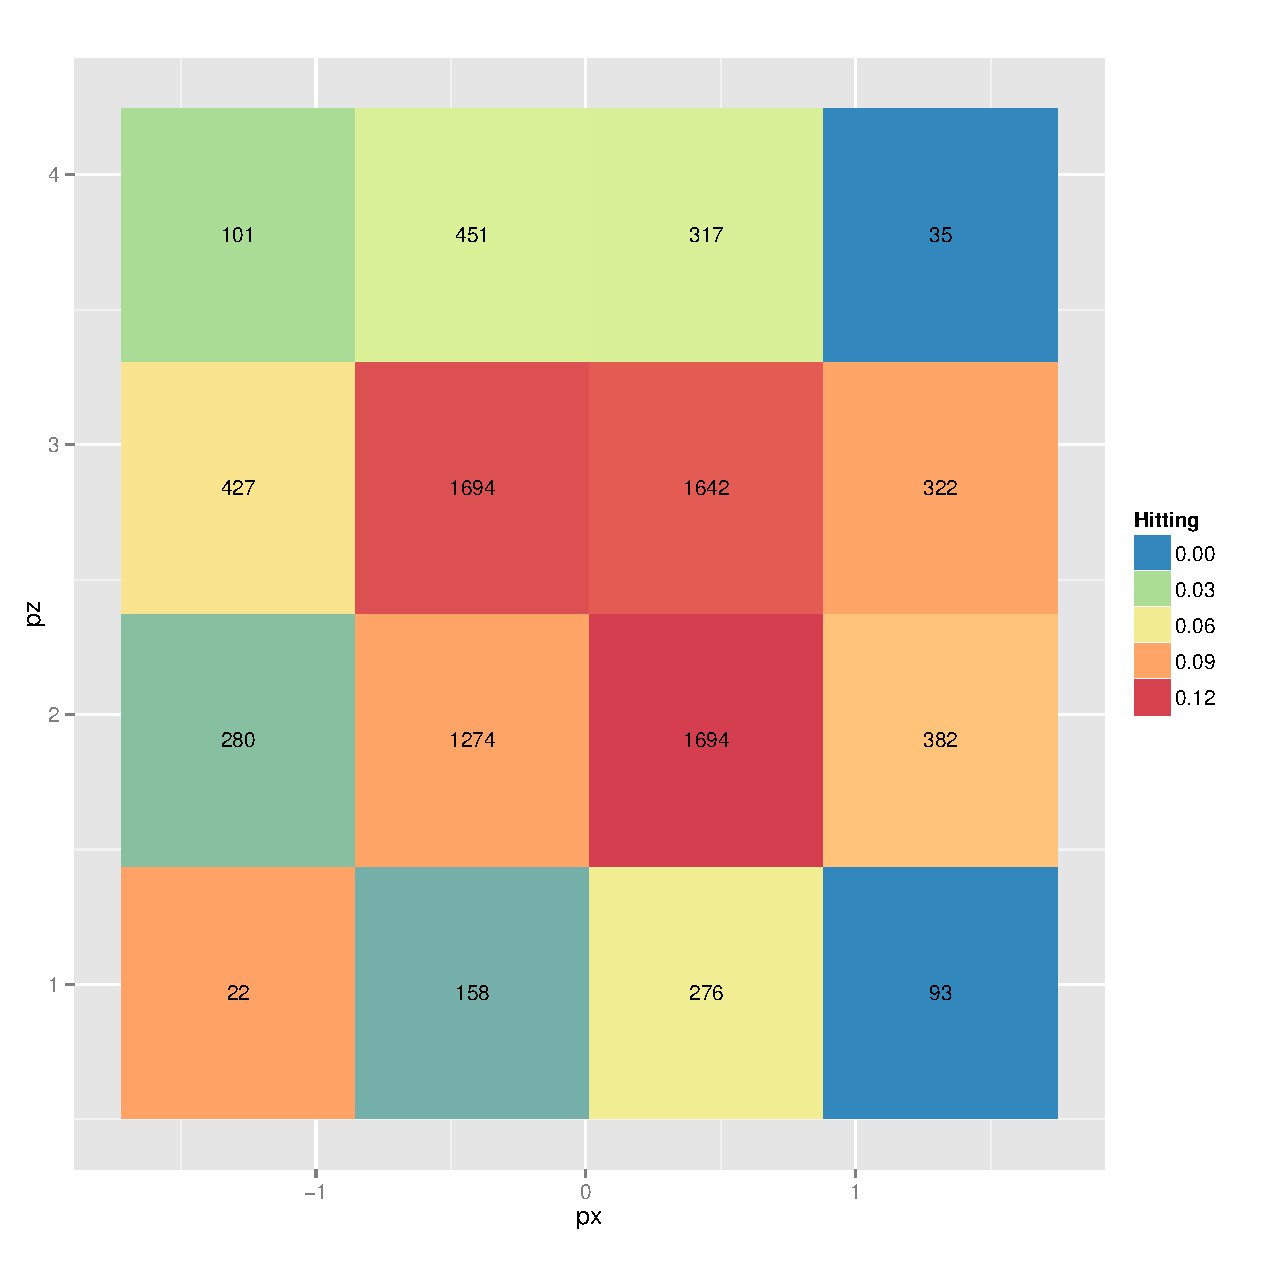
\includegraphics[scale=.3]{Images/Chapter4x4.pdf} 
      	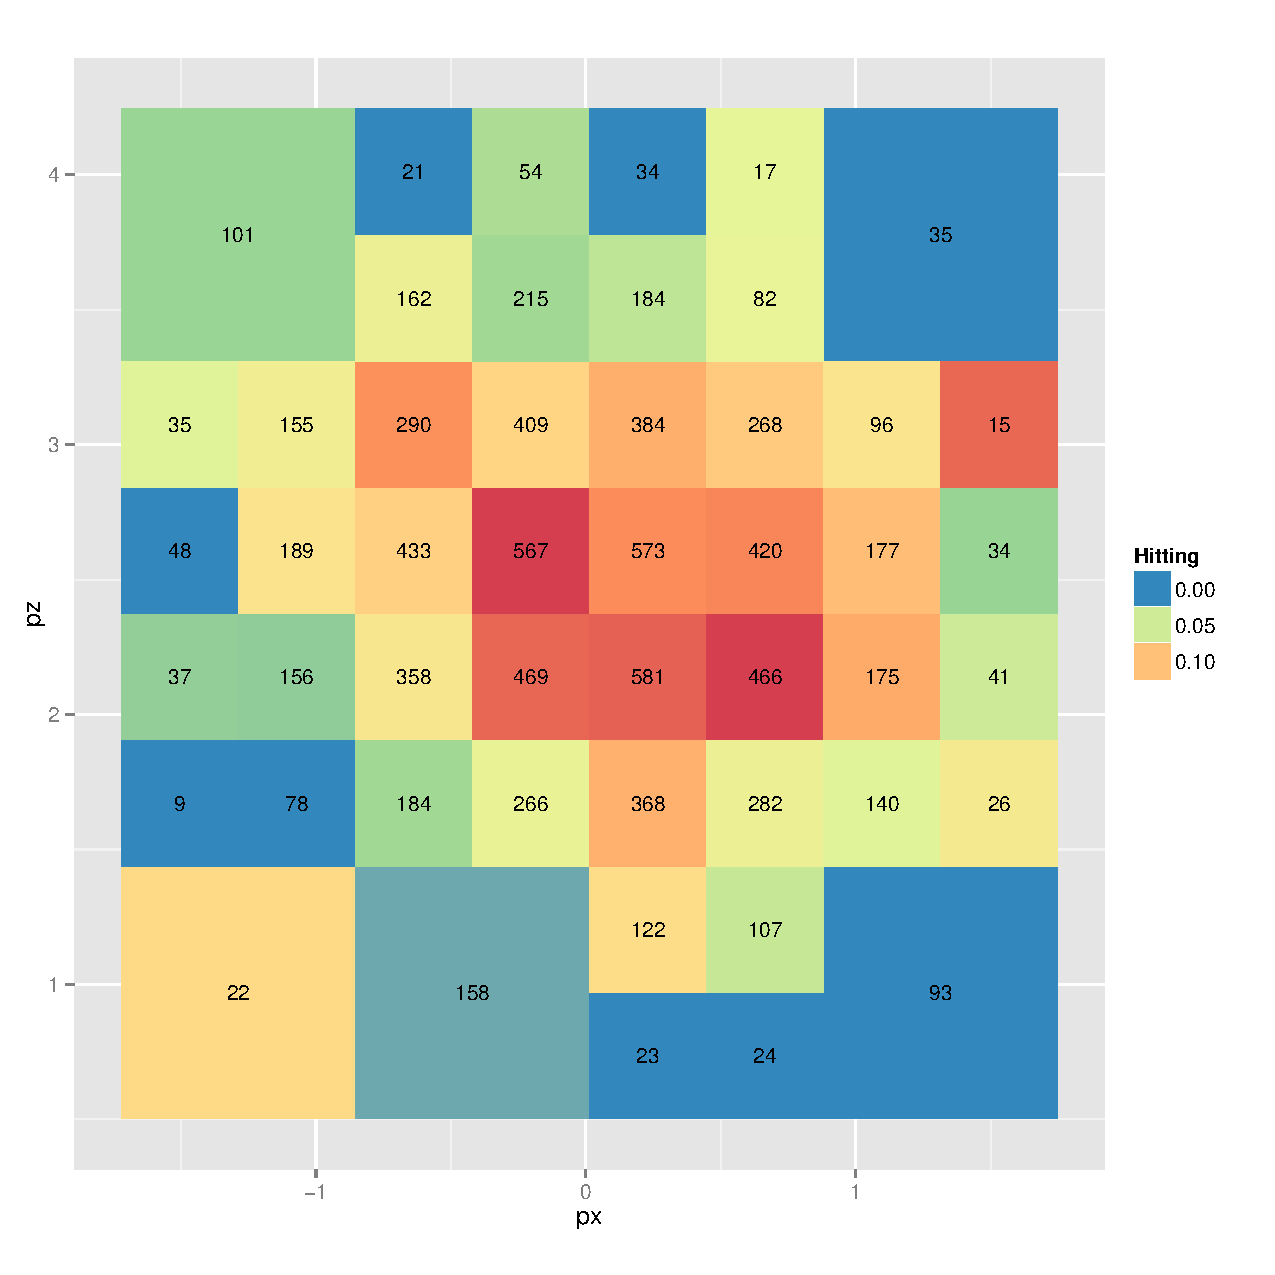
\includegraphics[scale=.3]{Images/Chapter8x8_200.pdf} 
      	\caption{These heat maps show the empirical hitting success probability of Johnny Peralta, for pitches passing through the space represented by each square region of the hitting zone.  Each box maps $\hat{p}_{b}$ to a color, with box sample sizes, $n_{b}$, printed on box centers. All boxes with a sample size greater than 200 in the heat map on the left, have been subdivided in the heat map on the right. Box 22, and others like it, remain intact because further subdivision yields uninformatively low sample sizes.}
      	\end{figure} 
      	
Notice all four corner boxes remain intact. This indicates Peralta  swings less often at pitches in the stike zone corners, and/or less often sees pitches in the corners of the strike zone. We delve into the possible reasons for this pattern, in baseball context, in Section 1.3.3.

Considering again features pertinent to further subdivision, sixteen boxes still contain a sample size greater than 200, and 11 still have a sample size greater than 300. We subdivide again, all 16 boxes where $n_{b} > 200$.
        \begin{figure}[H]
      	\centering
      	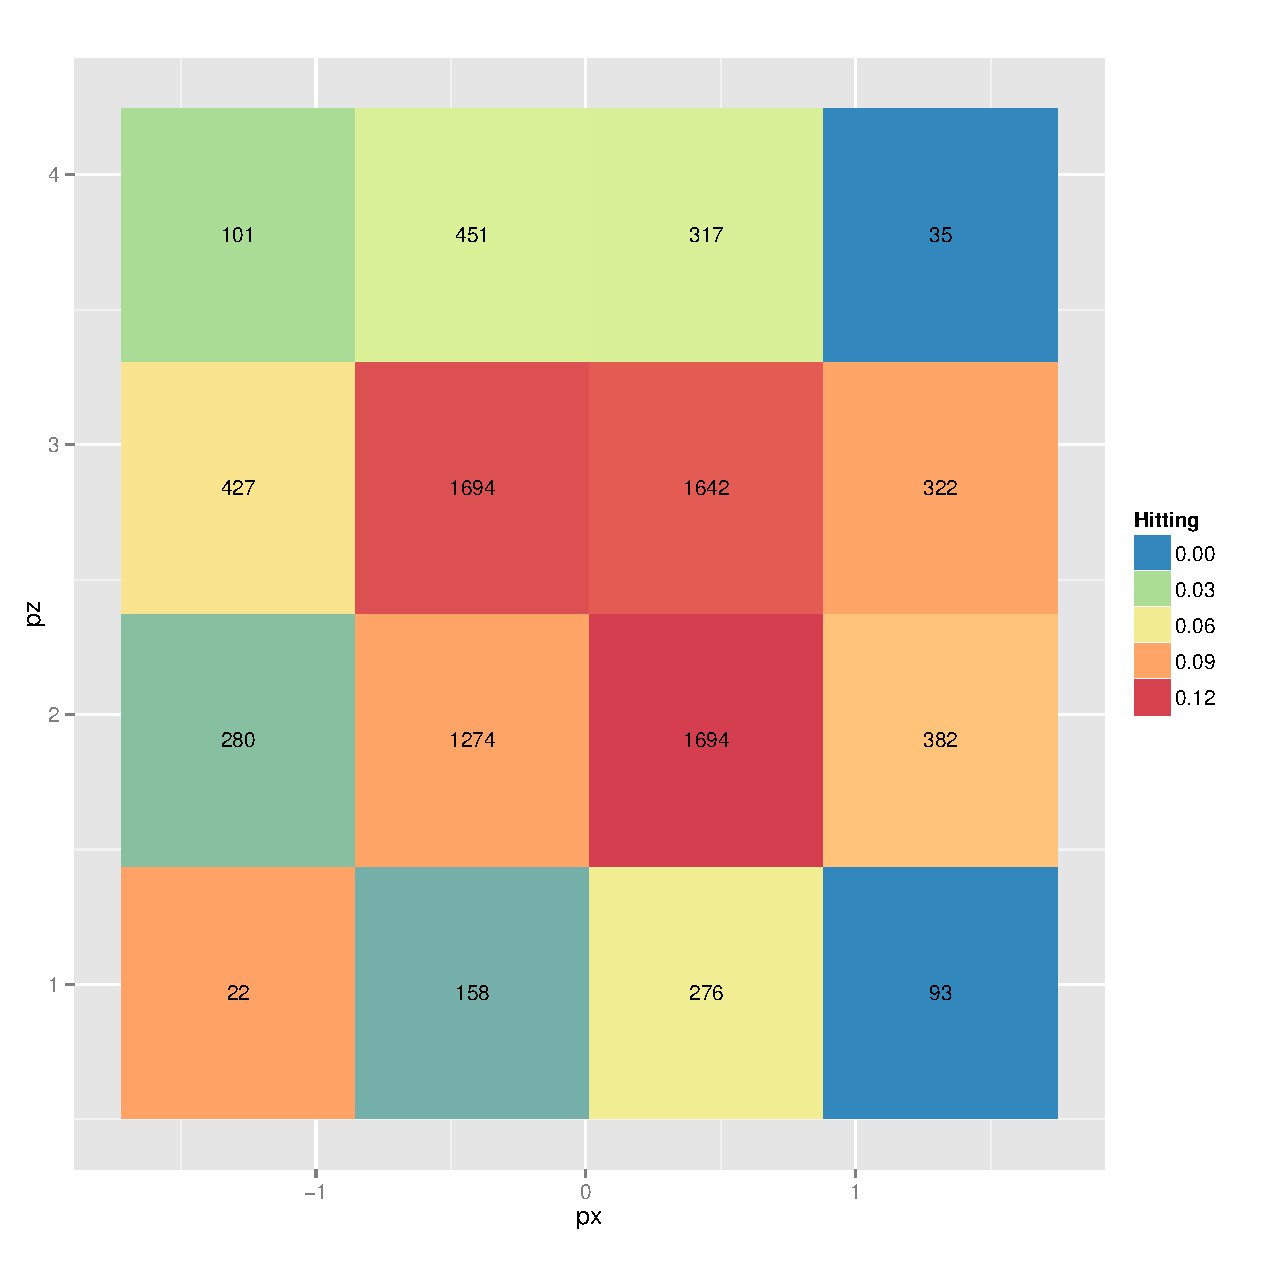
\includegraphics[scale=.22]{Images/Chapter4x4.pdf}
      	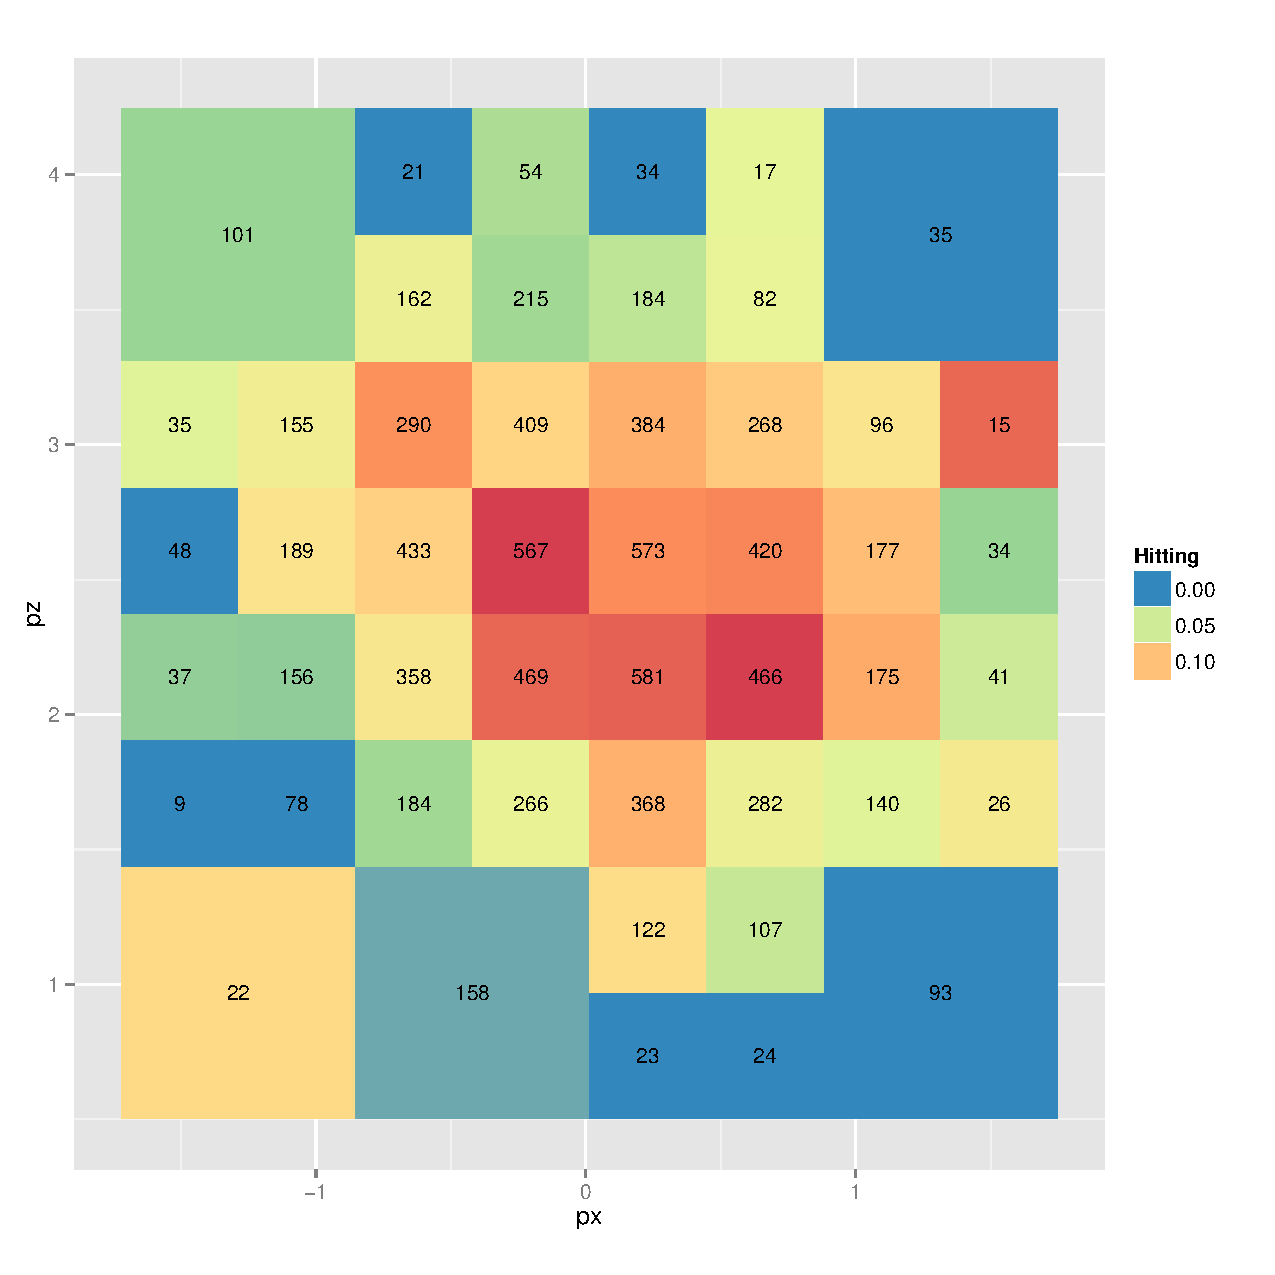
\includegraphics[scale=.22]{Images/Chapter8x8_200.pdf} 
      	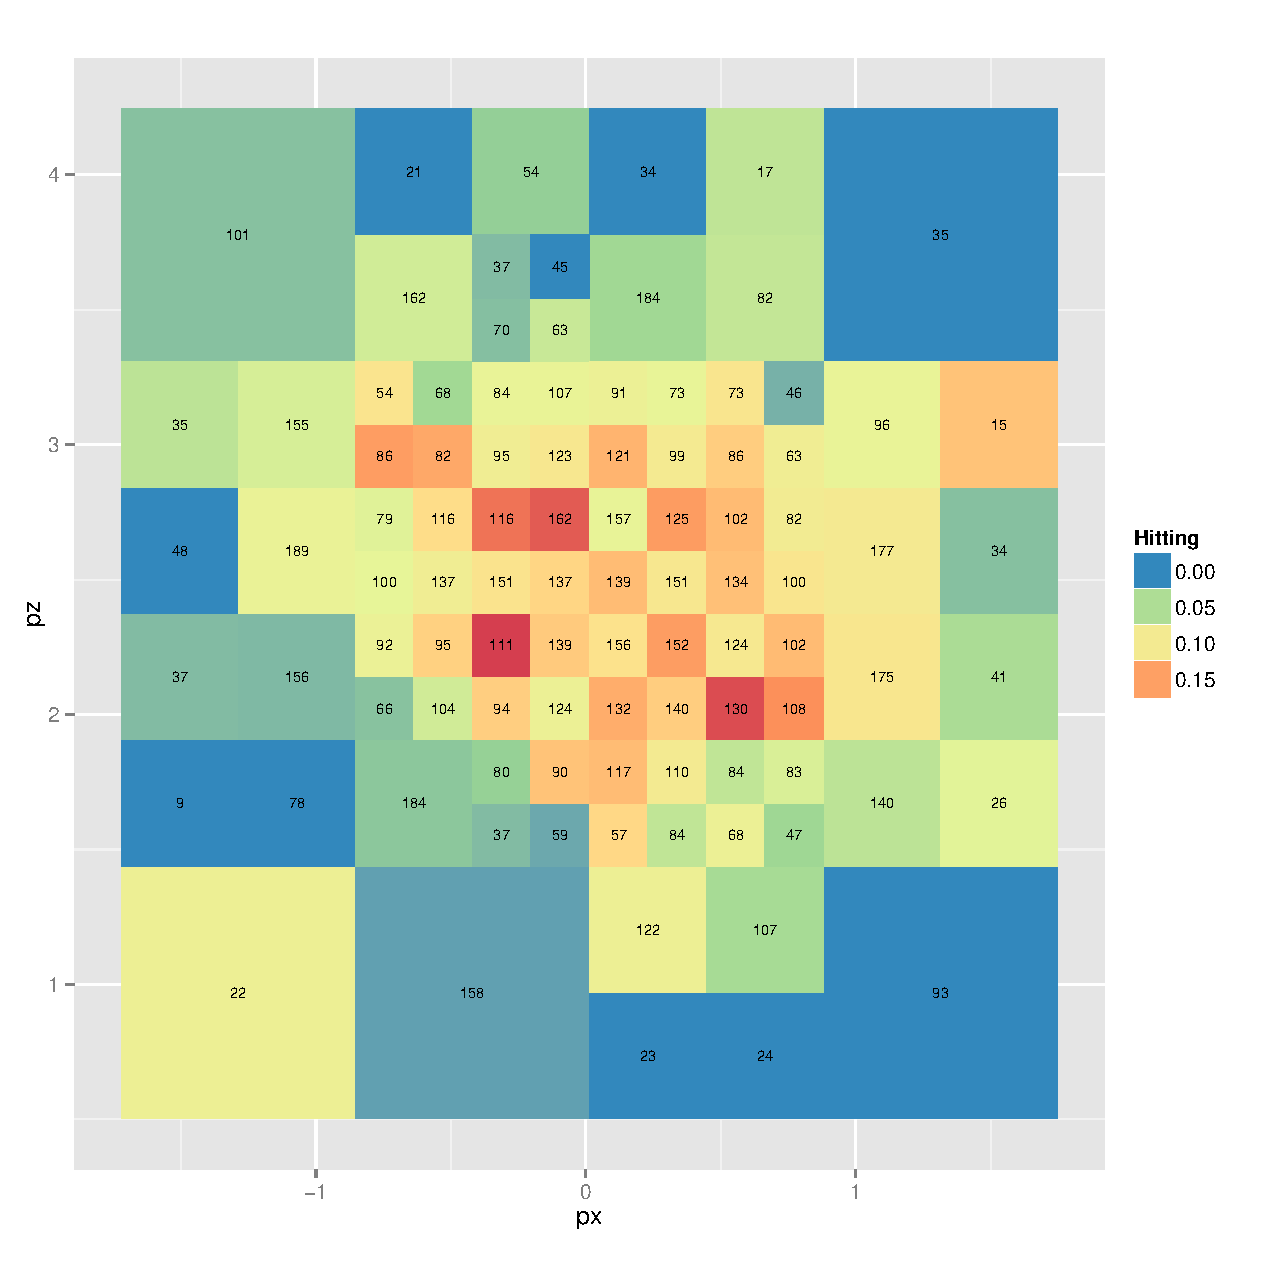
\includegraphics[scale=.22]{Images/Chapter16x16_200.pdf} 
      	\caption{(BIGGER COUNTS) Two iterations in the varying-resolution algorithm. These heat maps convey the empirical batting average of batter 425509, Johnny Peralta, in each boxed region of the hitting zone. Each box maps $\hat{p}_{b}$ to a color. The number printed on each box represents the number of pitches the hitter swung at that passed through that box. All boxes with a sample size greater than 200 in the heat map on the left, have been subdivided in the heat map in the middle. All boxes with a sample size greater than 200 in the heat map in the middle, have been subdivided in the heat map on the right.}
      	\end{figure}
The left-hand and middle heat maps in Figure 1.6 reproduce Figure 1.5. Notice the middle heat map in Figure 1.6 contains 16 boxes with $n_{b} > 200$. We subdivide these 16 boxes, each into four smaller, equally sized boxes; yielding the right-hand map. The right-hand heat map consists of 97 boxes, with a mean box sample size of 94.57, and median of 94. Box 9 contains the fewest observations, and box 189 contains the most. Box 63 serves as the first quartile, while box 125 serves as the third quartile. 

In variable resolution heat maps, box size corresponds to data density. Figure 1.7 demonstrates this correspondence. 
        \begin{figure}[H]
      	\centering
      	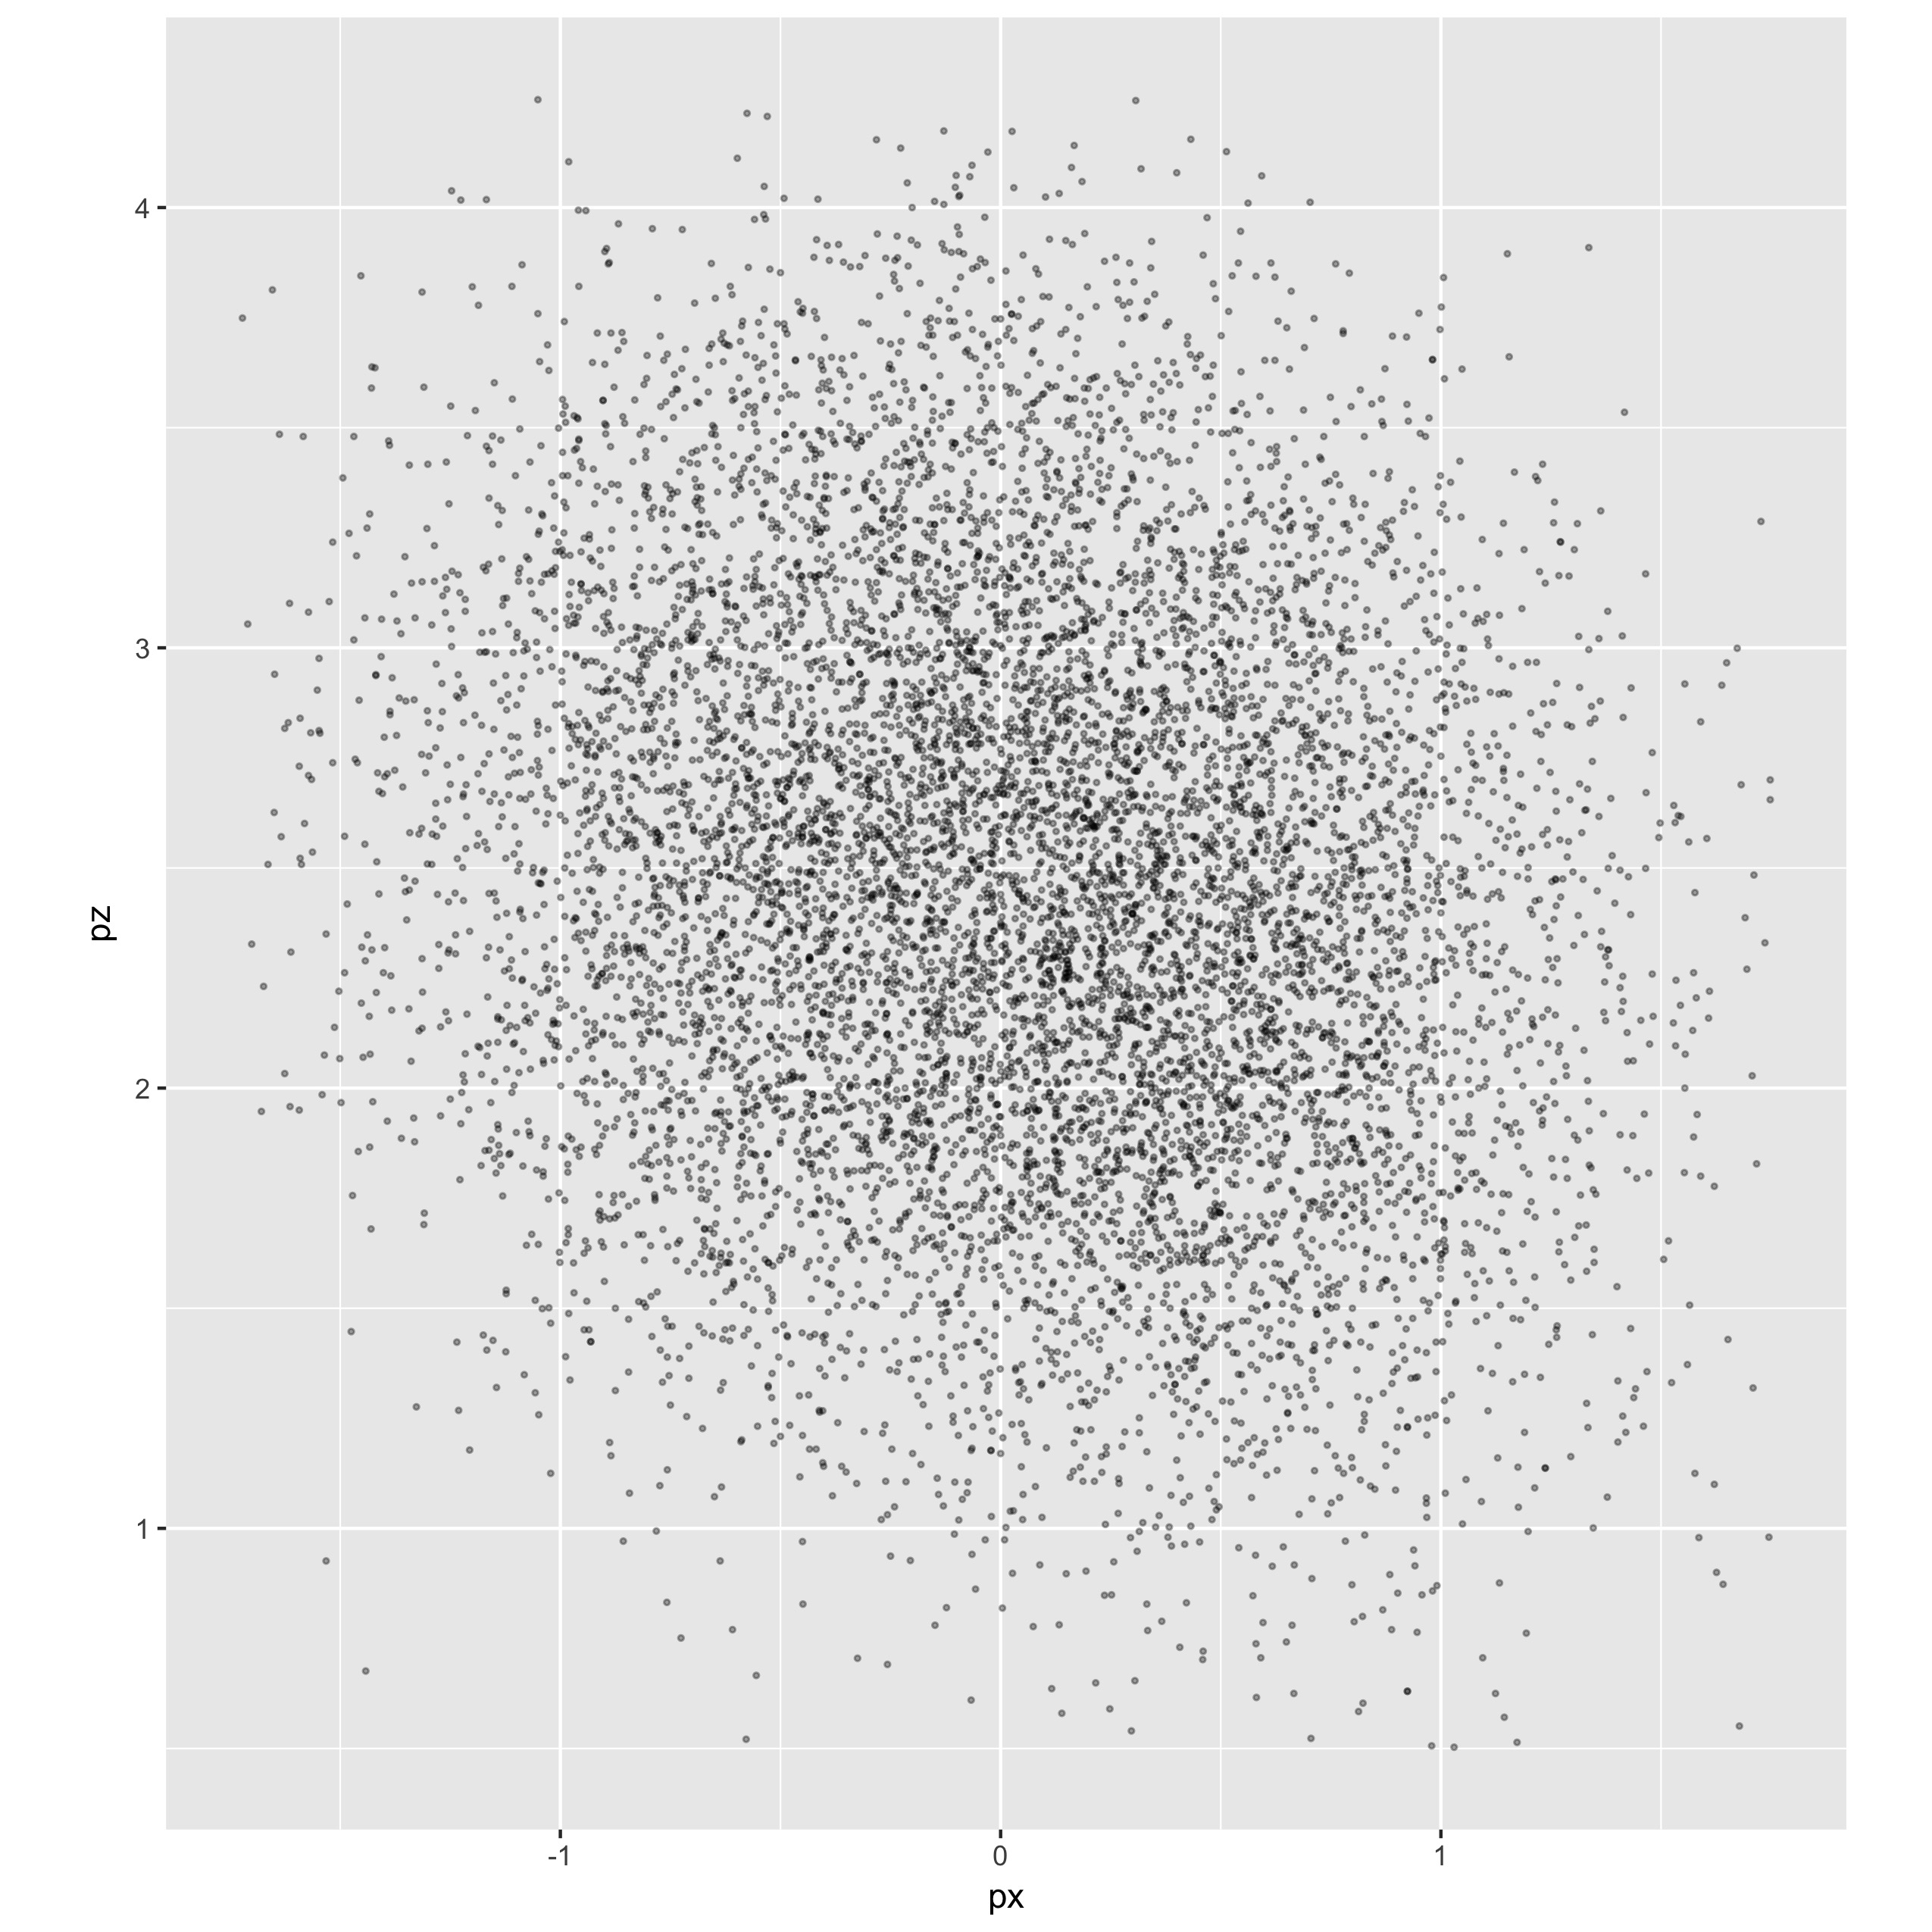
\includegraphics[scale=.07]{Images/density.jpg}
      	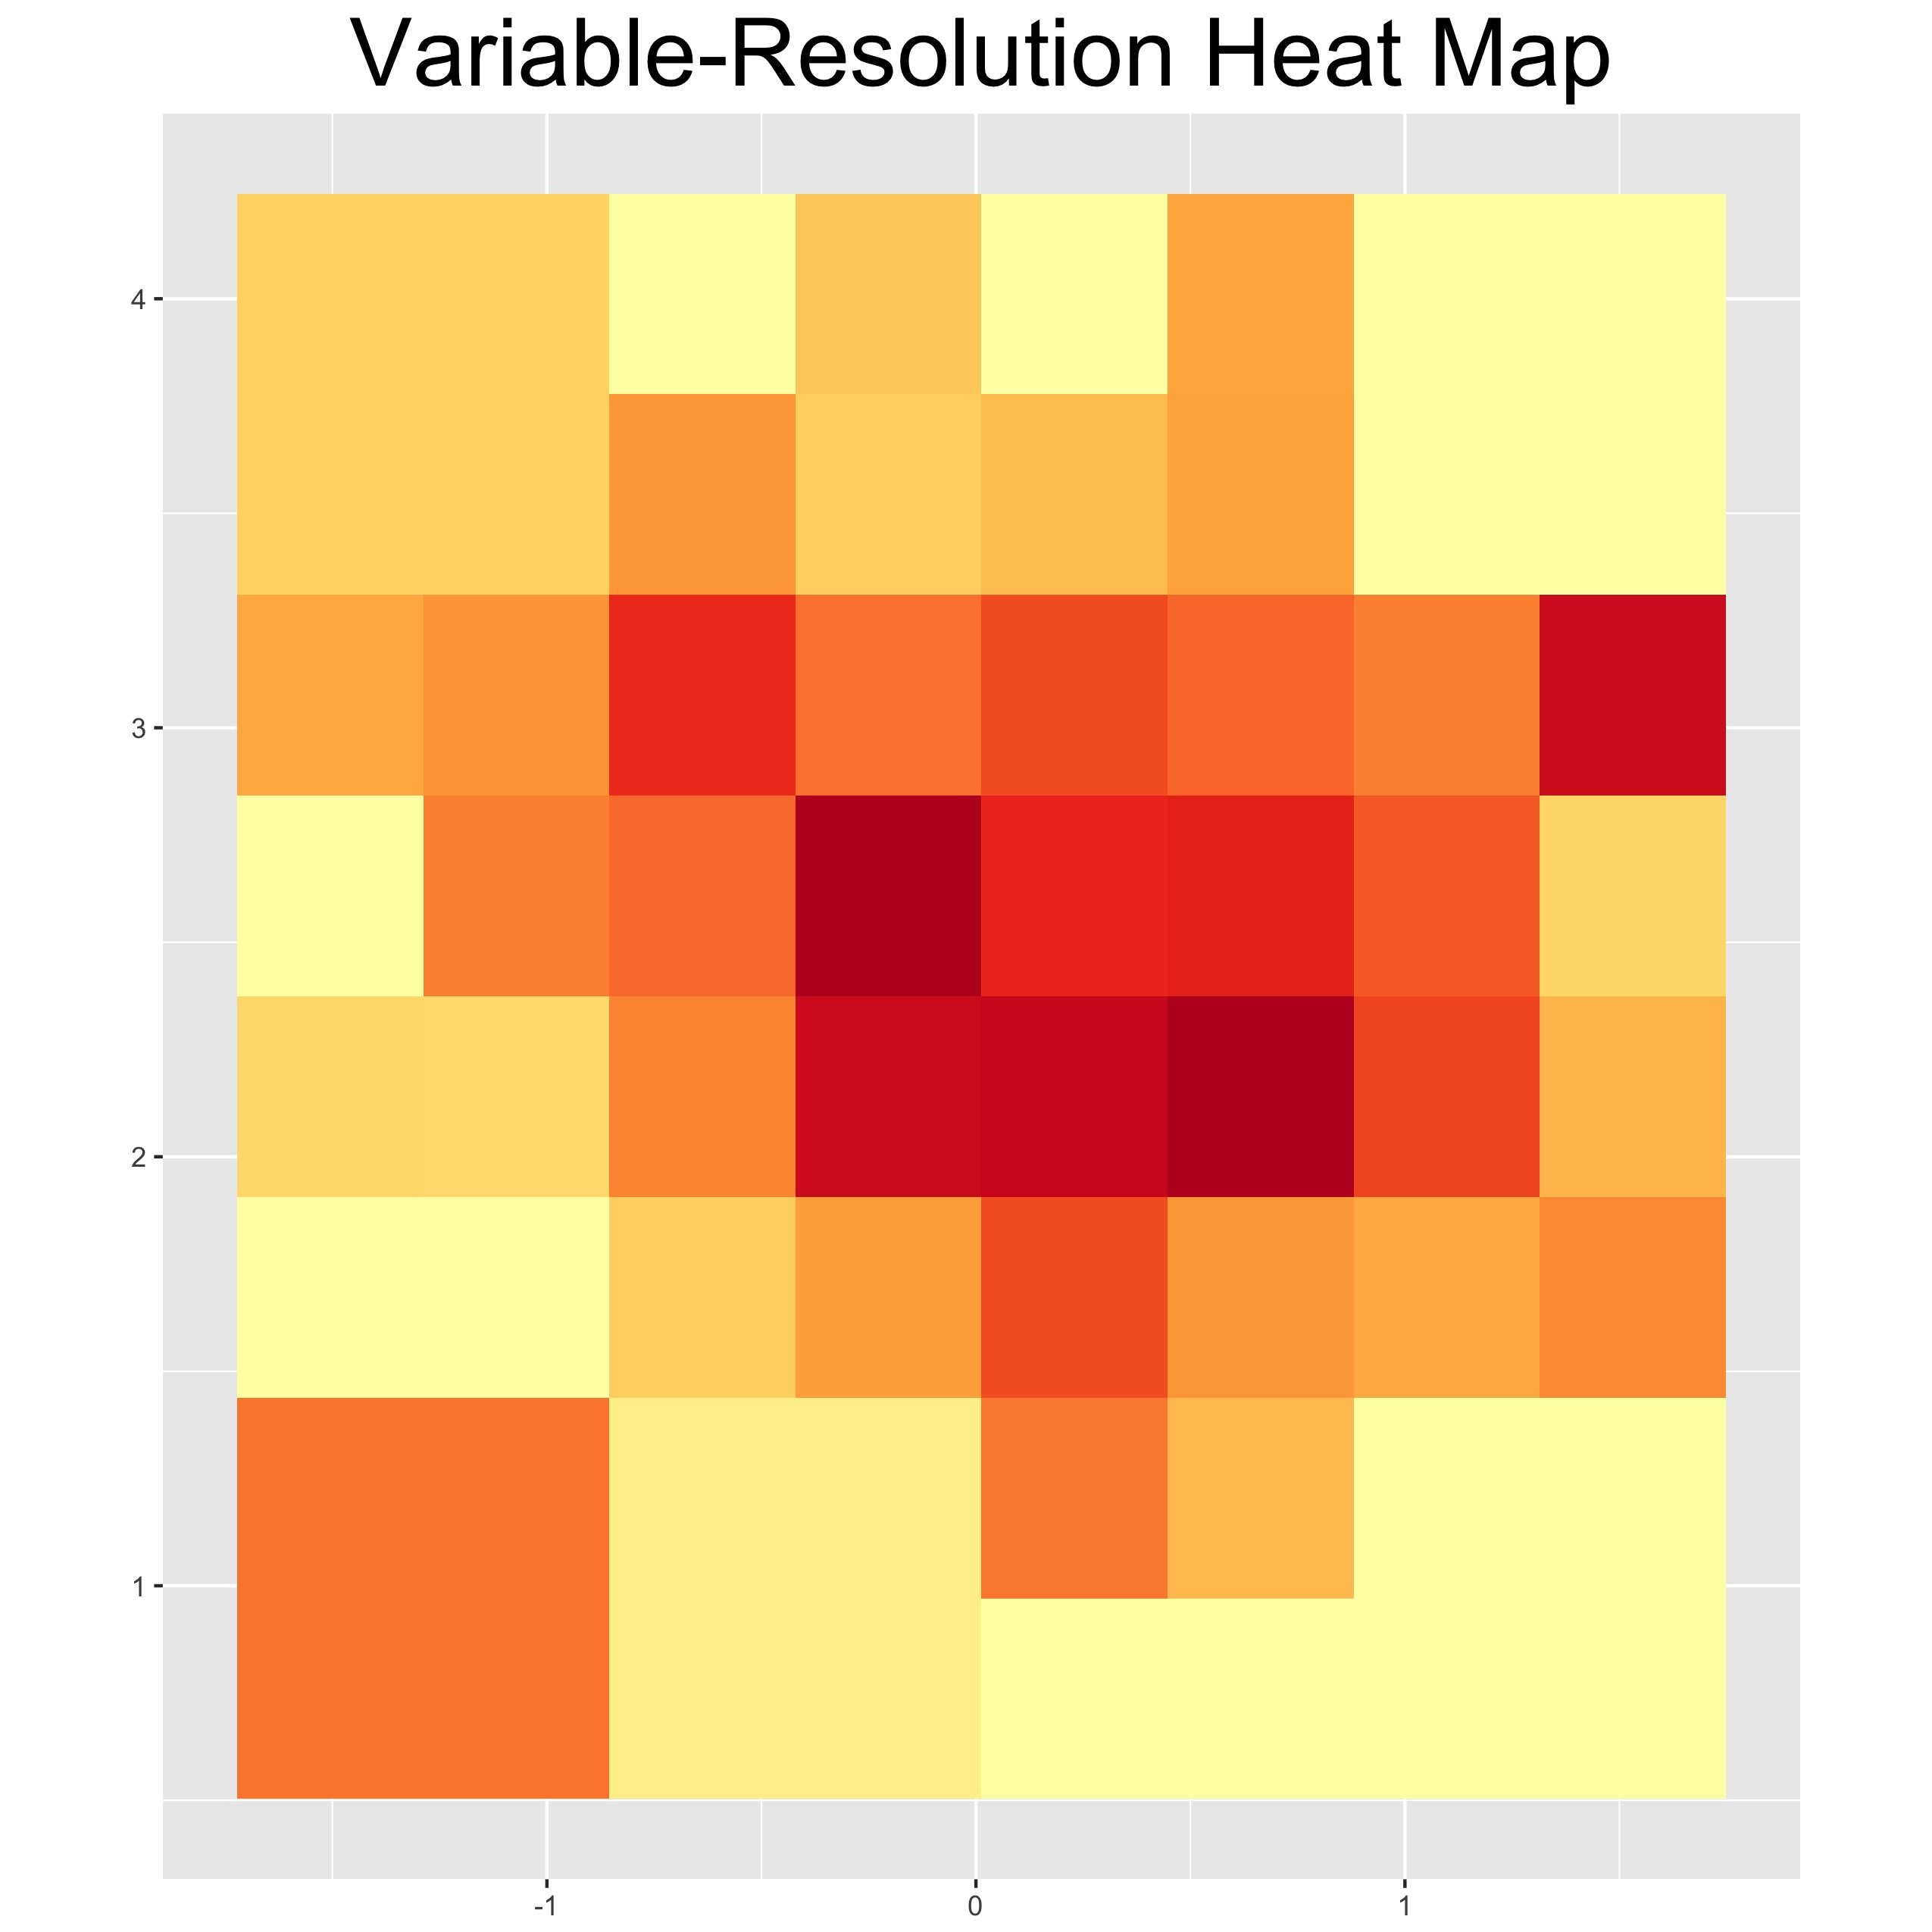
\includegraphics[scale=.07]{Images/density_comp.jpg} 
      	\caption{A scatterplot and a variable-resolution heat map of Johnny Peralta's empirical, spatial hitting success probabilities. The finer resolution regions in the heat map correspond to greater data density, as demonstrated in the scatterplot. Traditional heat maps omit this information.}
      	\end{figure}
Notice how smaller boxes inidicate greater density of pitch-swings, while larger boxes relect lower density of pitch-swings. This contrasts favorably to a traditional heat maps, whose uniform resolution hides data density. Variable-resolution heat maps convey valuable, previously omitted data density information to the viewer. This marks a noteworthy improvement over tradiional heatmaps.

Figure 8 gives the full sequence of heat maps that result from applying the stopping rule $n_{b} < 200$, starting with a single box.
        \begin{figure}[H]
      	\centering
      	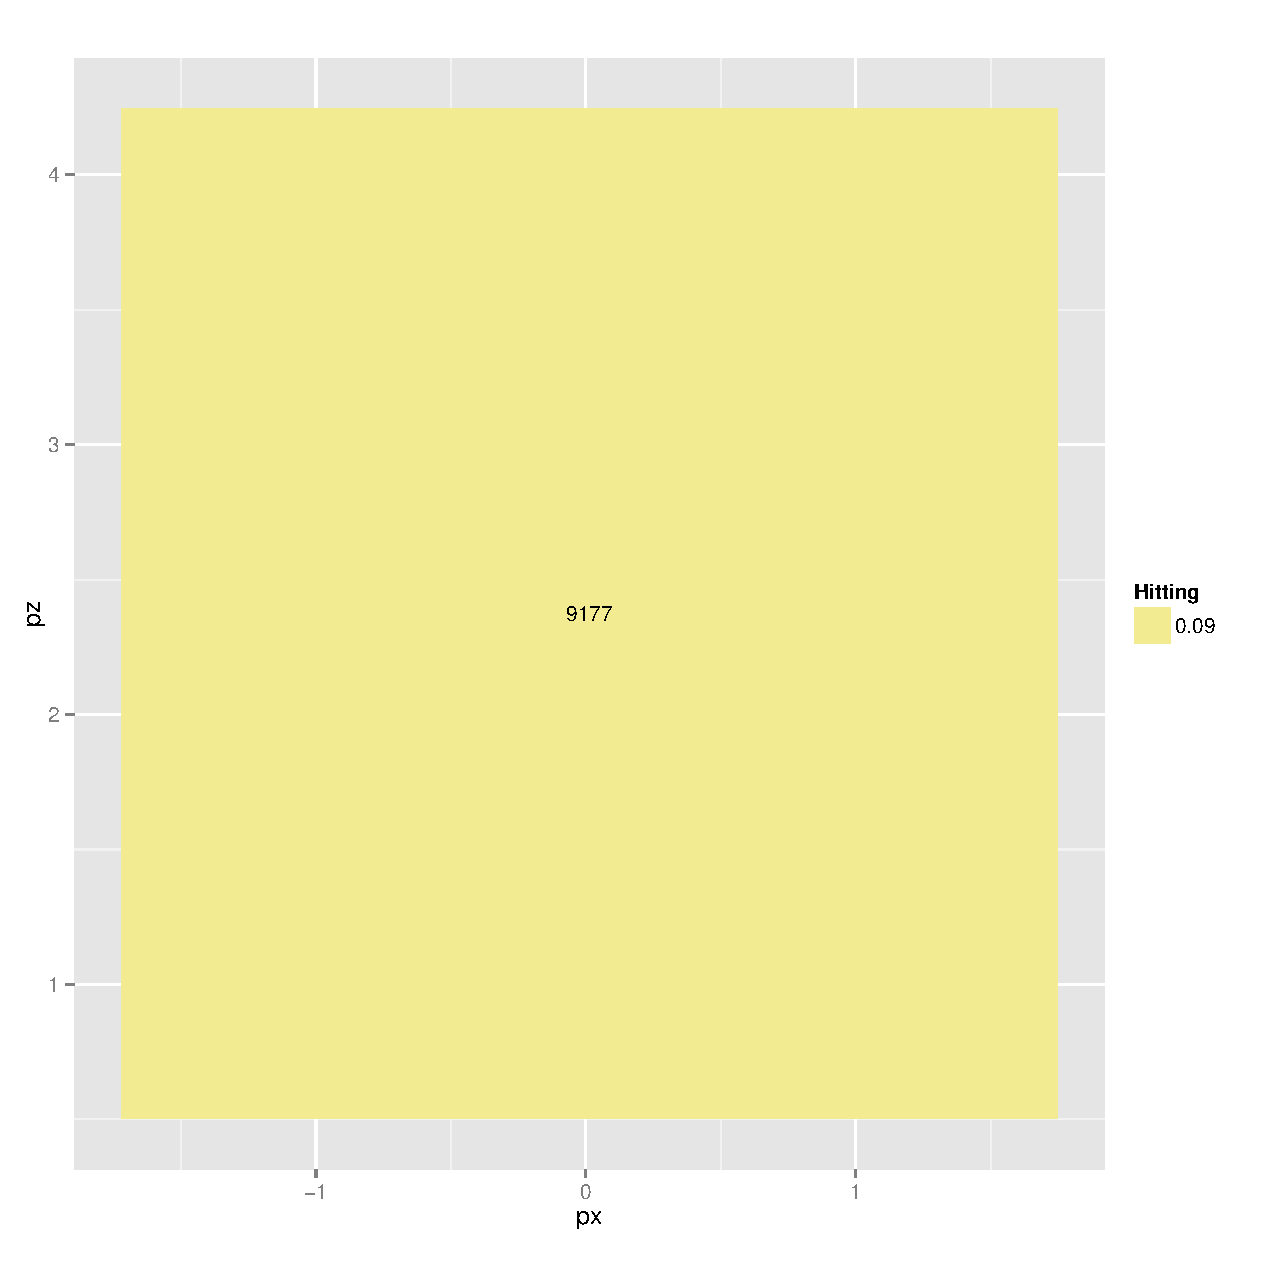
\includegraphics[scale=.2]{Images/Chapter1x1.pdf}
      	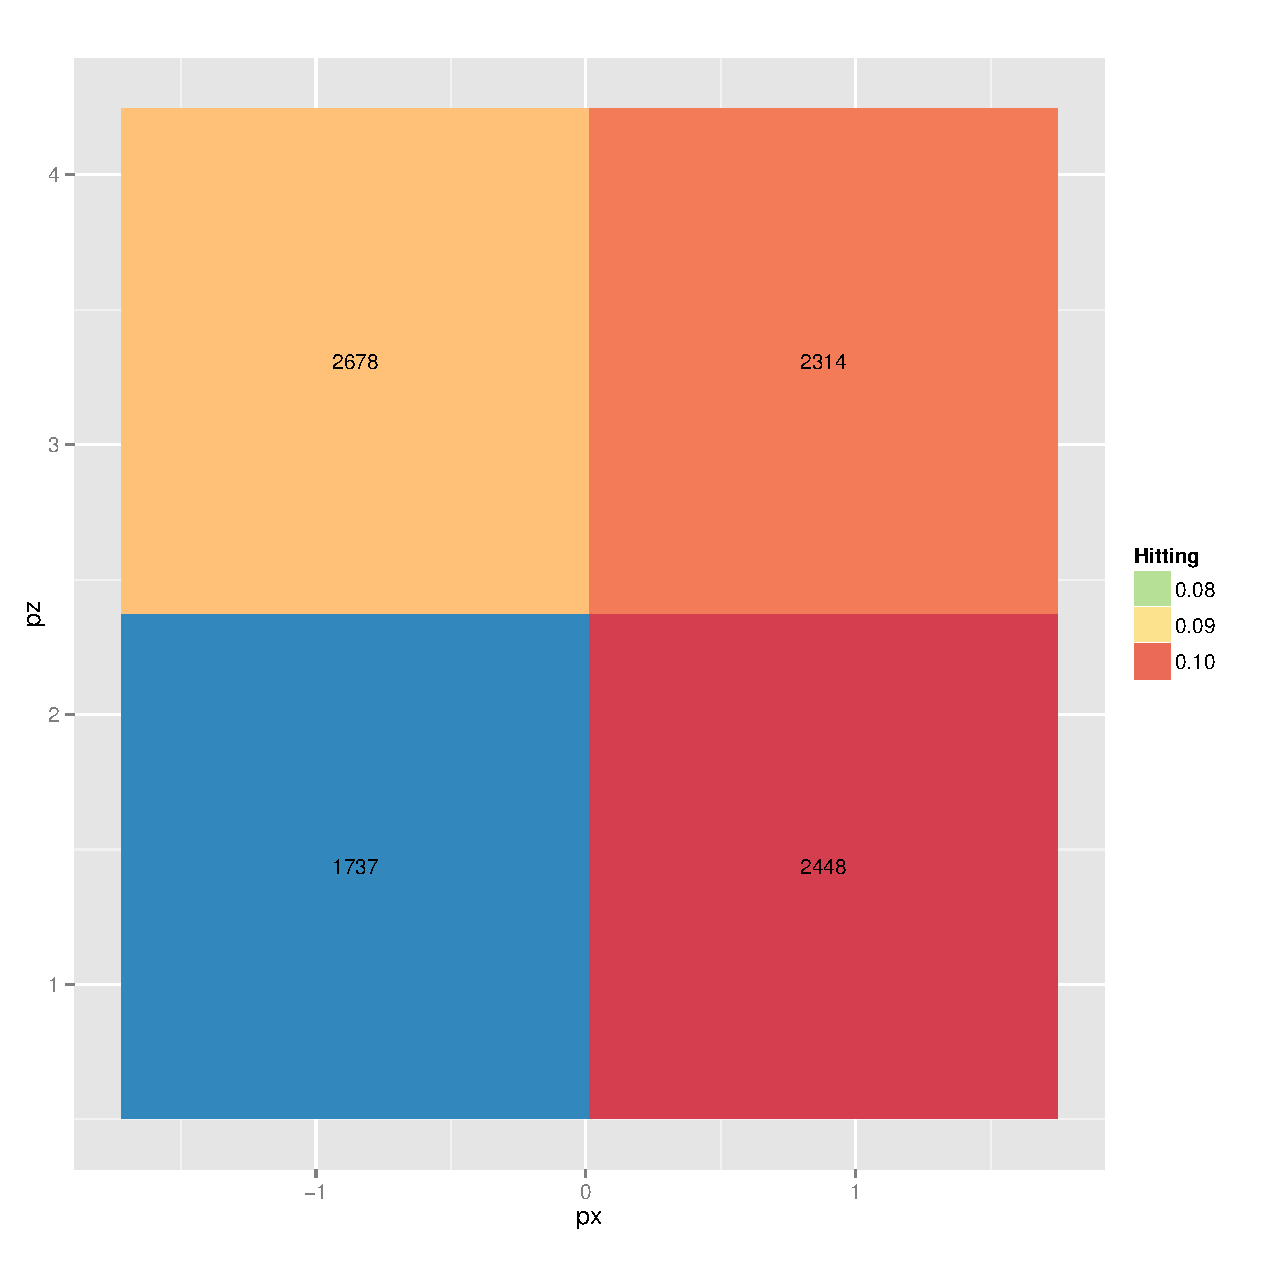
\includegraphics[scale=.2]{Images/Chapter2x2.pdf}
      	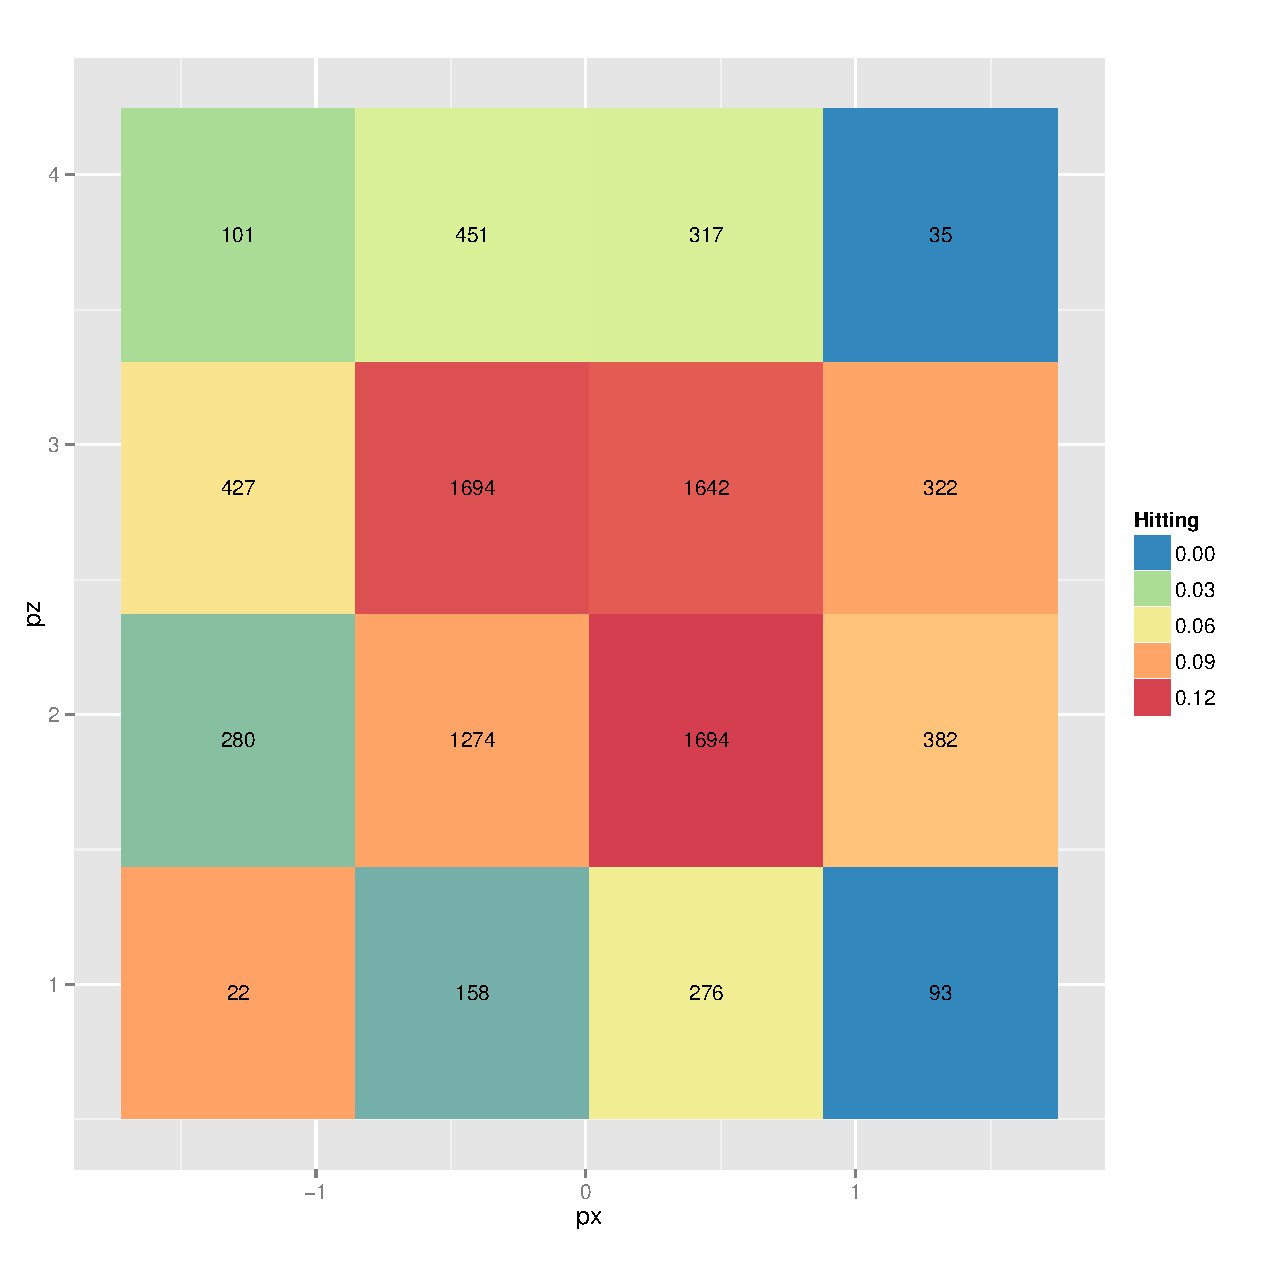
\includegraphics[scale=.2]{Images/Chapter4x4.pdf}
      	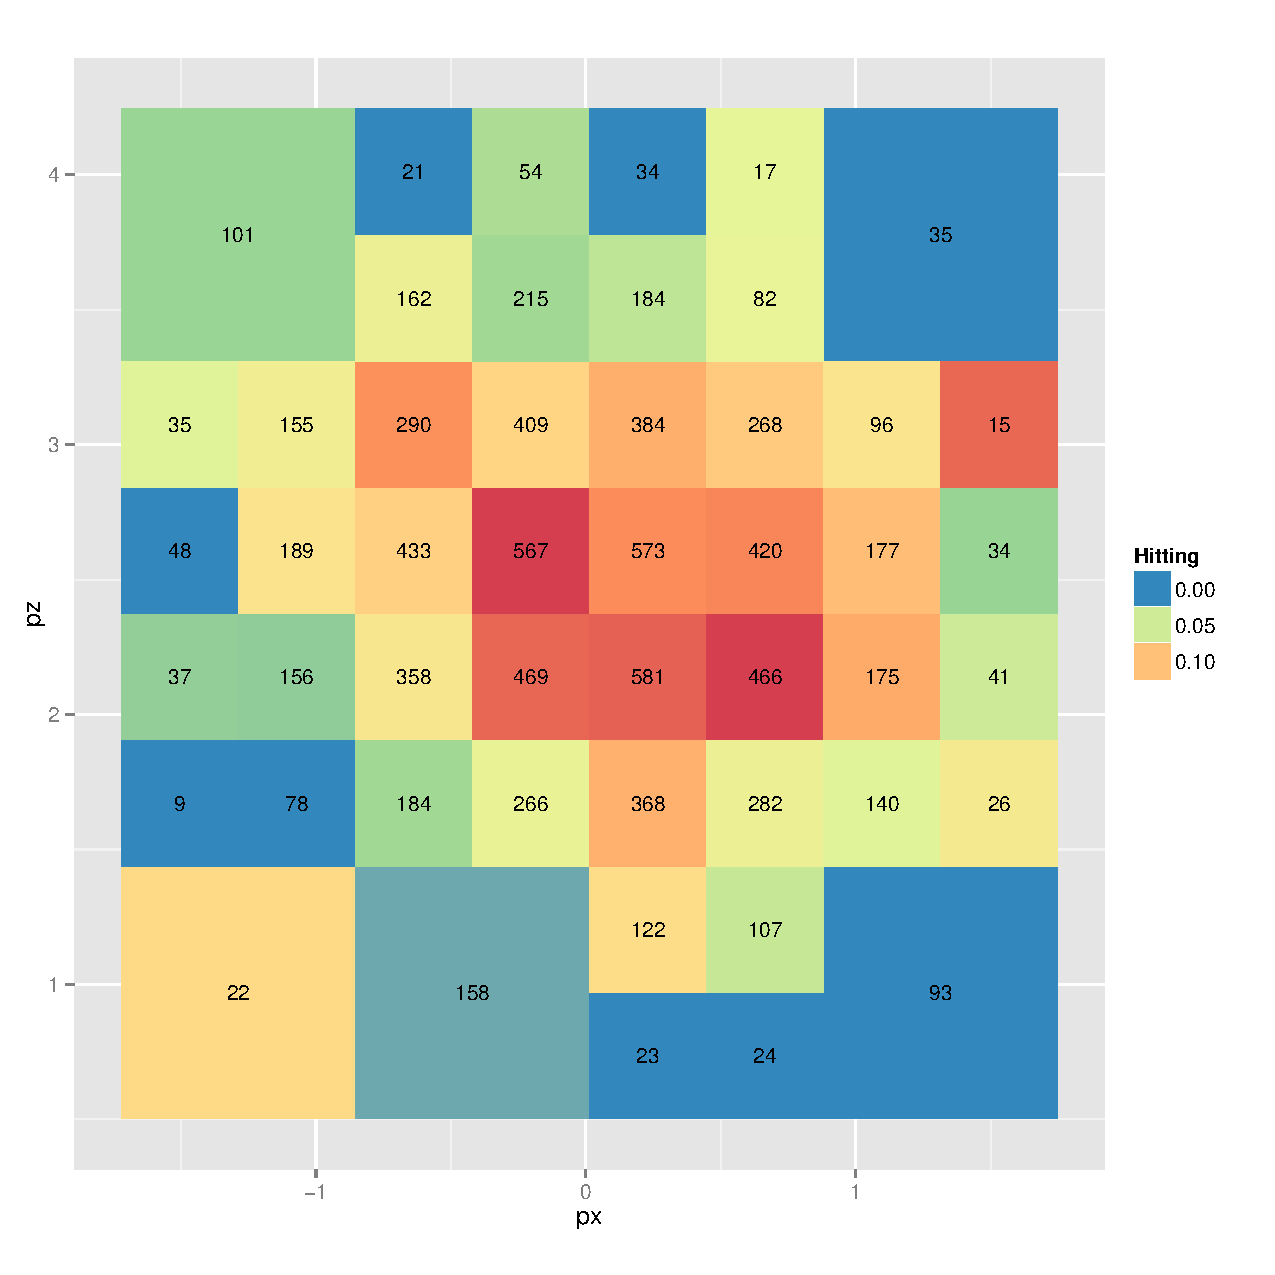
\includegraphics[scale=.2]{Images/Chapter8x8_200.pdf} 
      	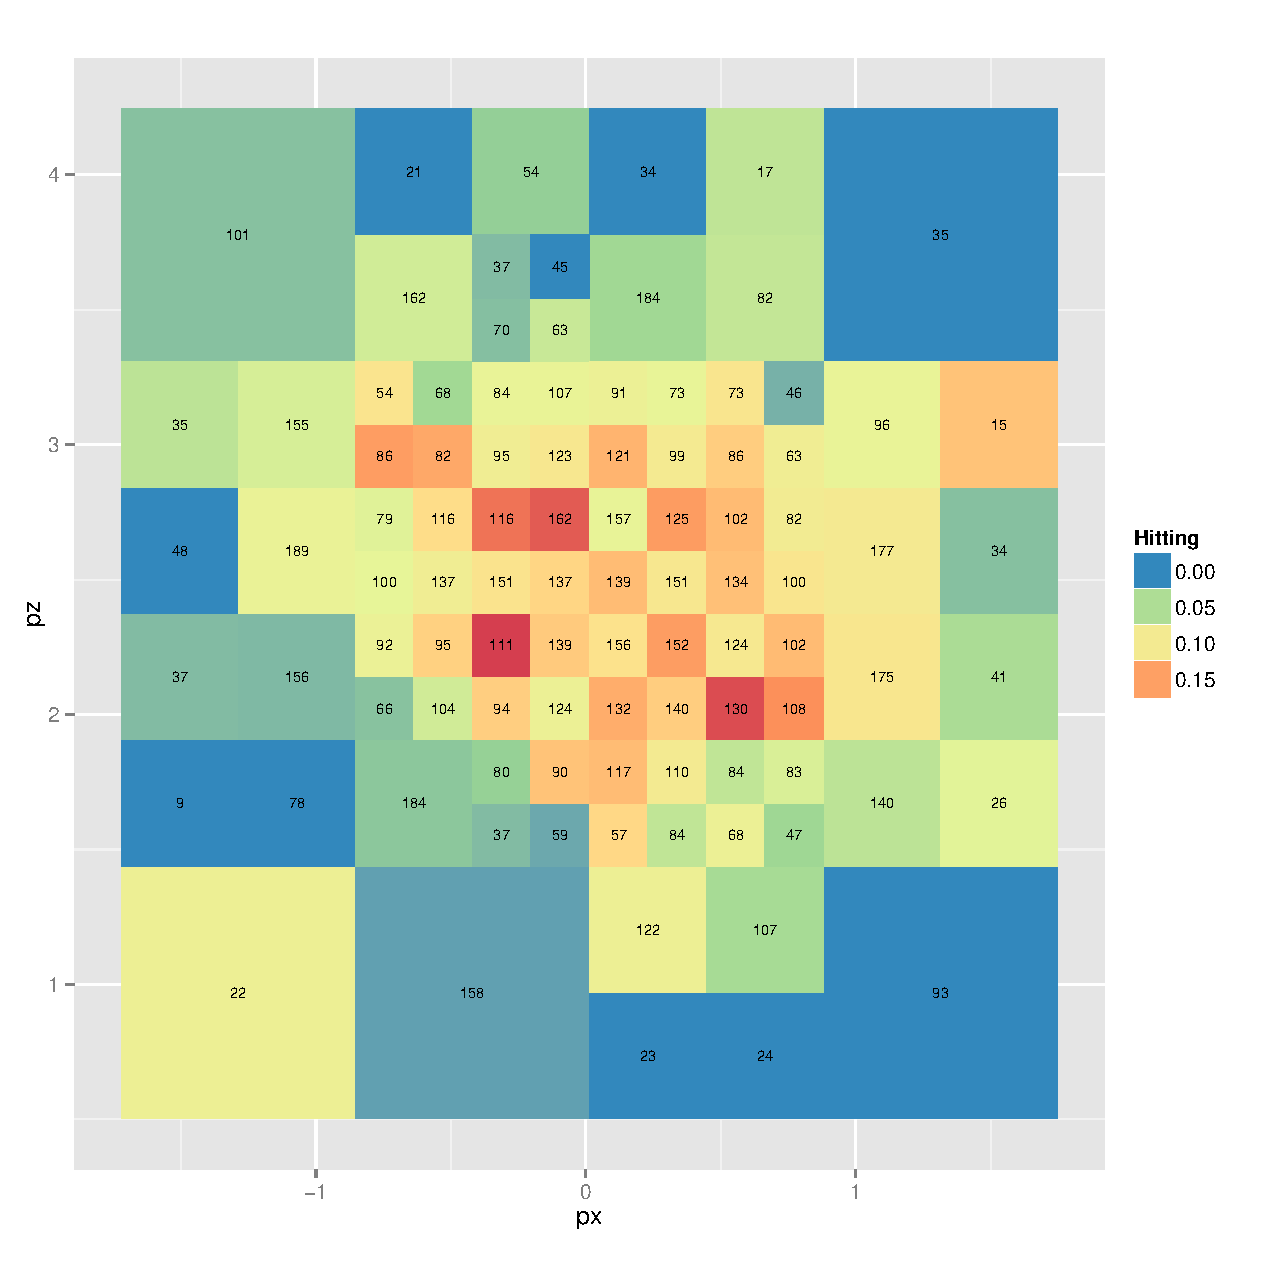
\includegraphics[scale=.2]{Images/Chapter16x16_200.pdf} 
      	\caption{These heat maps convey the empirical batting average of batter 425509, Johnny Peralta, in each boxed region of the hitting zone. Each box maps $\hat{p}_{b}$ to a color. The number printed on each box represents the number of pitches the hitter swung at that passed through that box. All boxes with a sample size greater than 200 in each heat map have been subdivided in the subsequent heat map.}
      	\end{figure}
      	
\subsection{Stopping Rule Example} % ===================
      	
To demonstrate the flexibility, consider a different stopping rule with the same subdivision algorithm. We subdivide boxes with $n_{b} > 100$, and Figure 1.9 gives the resulting sequence of heat maps.
        \begin{figure}[H]
      	\centering
      	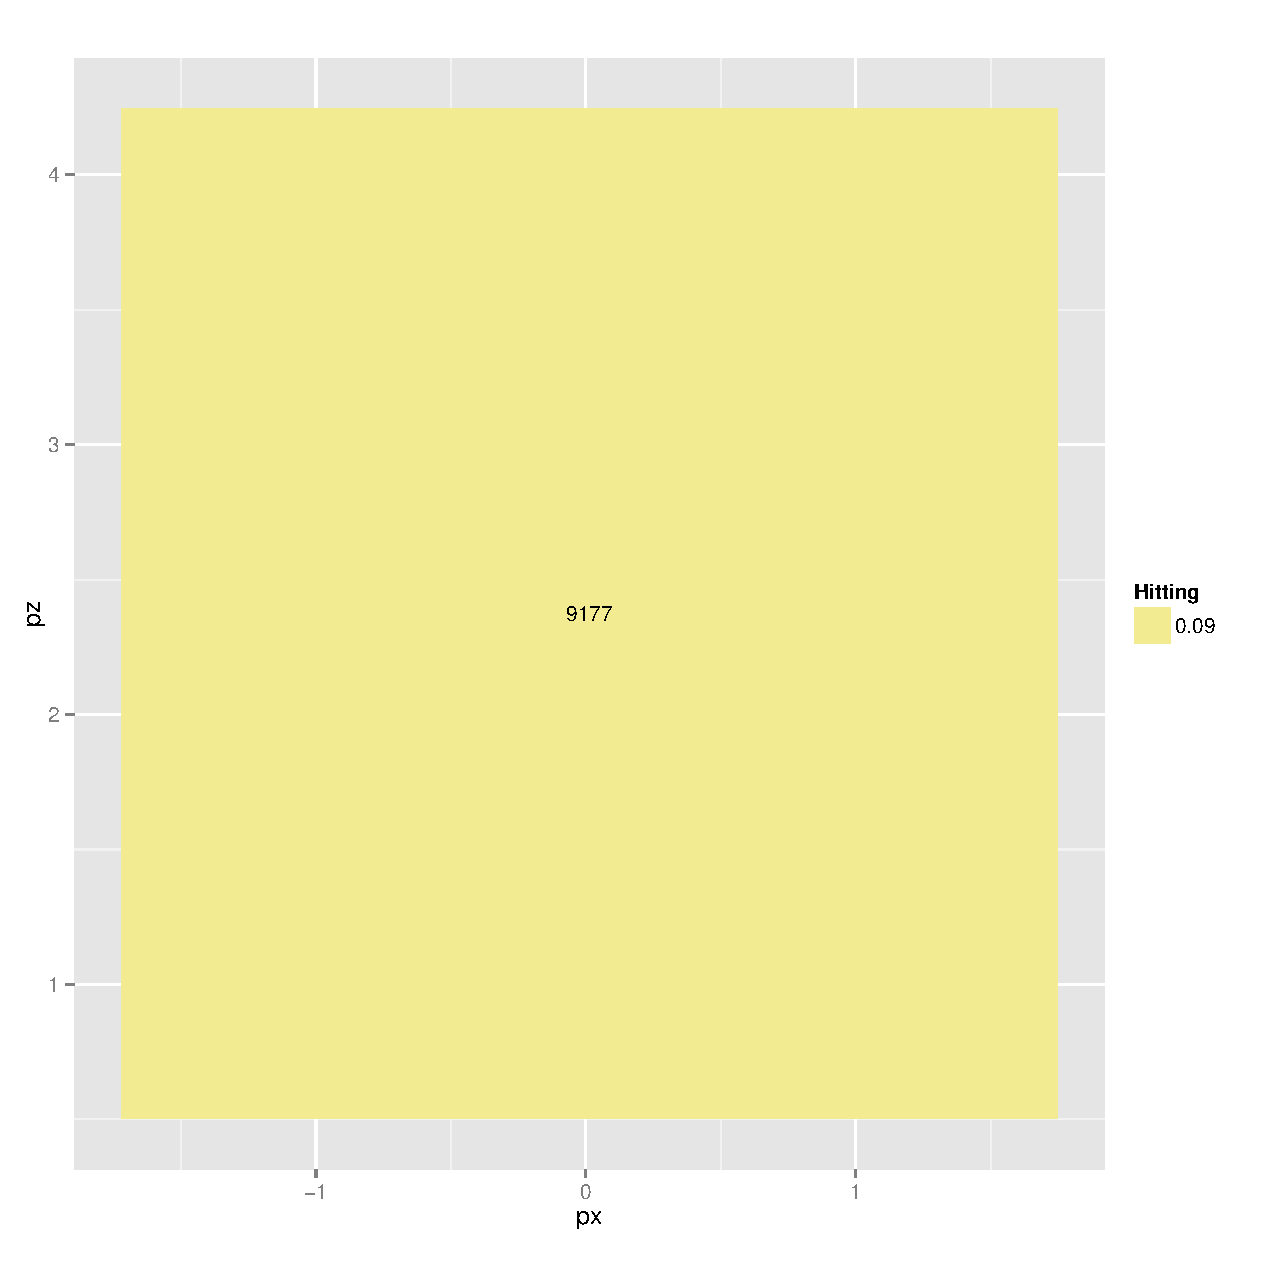
\includegraphics[scale=.2]{Images/Chapter1x1.pdf}
      	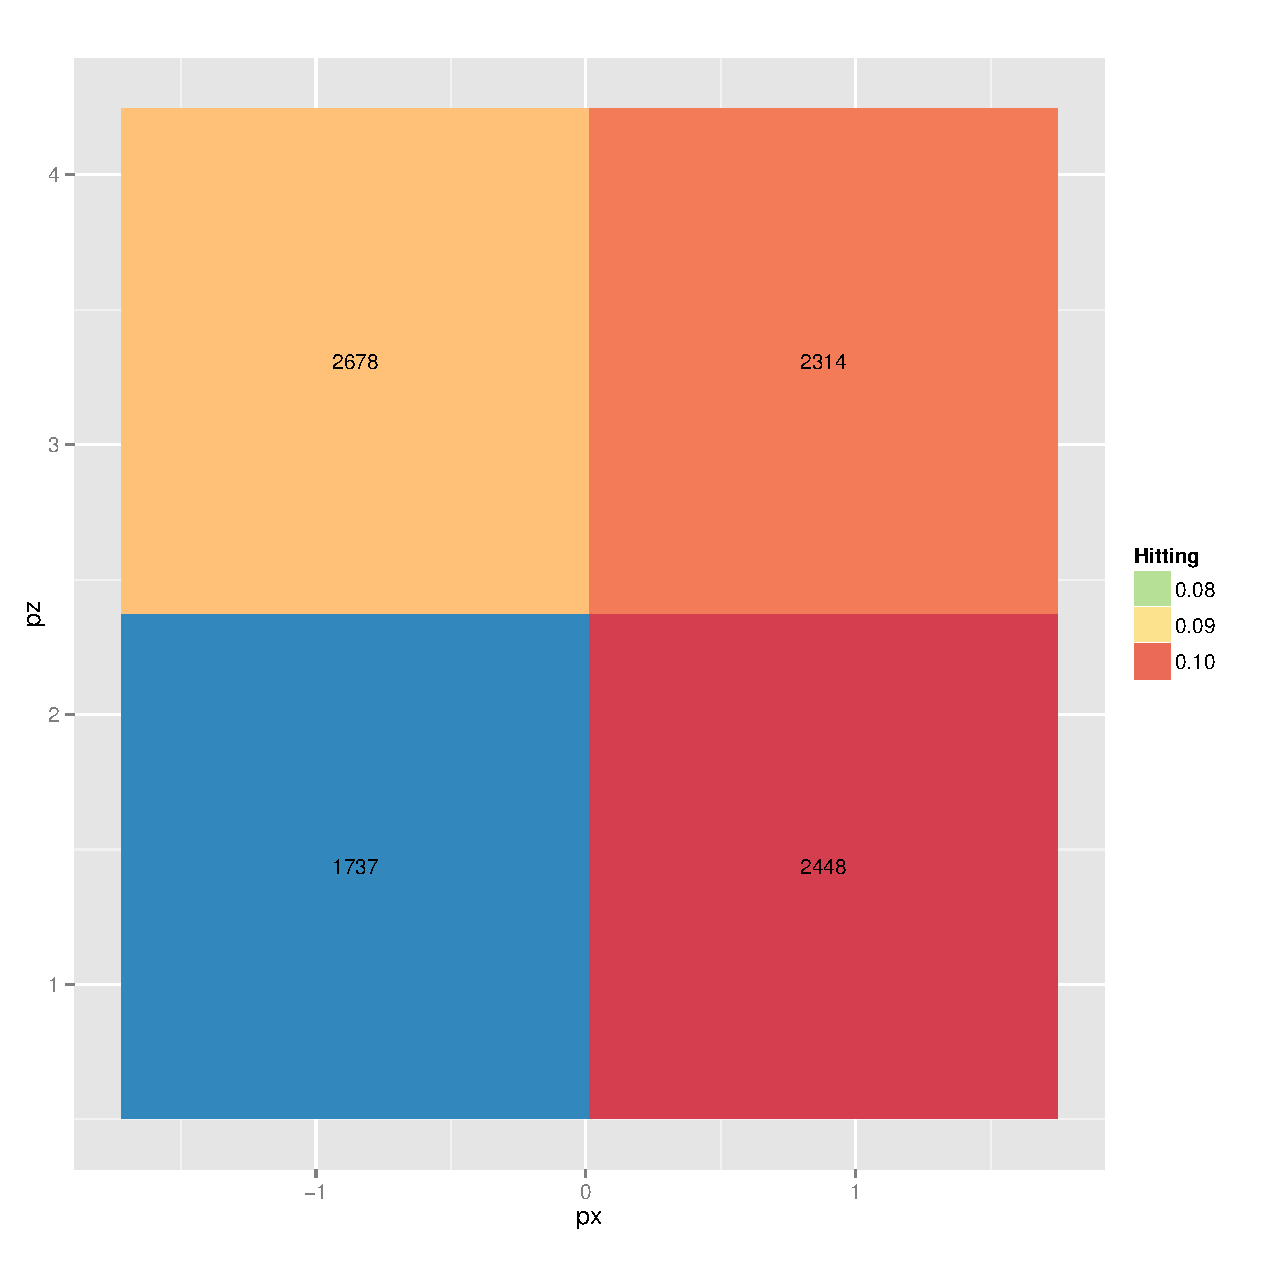
\includegraphics[scale=.2]{Images/Chapter2x2.pdf}
      	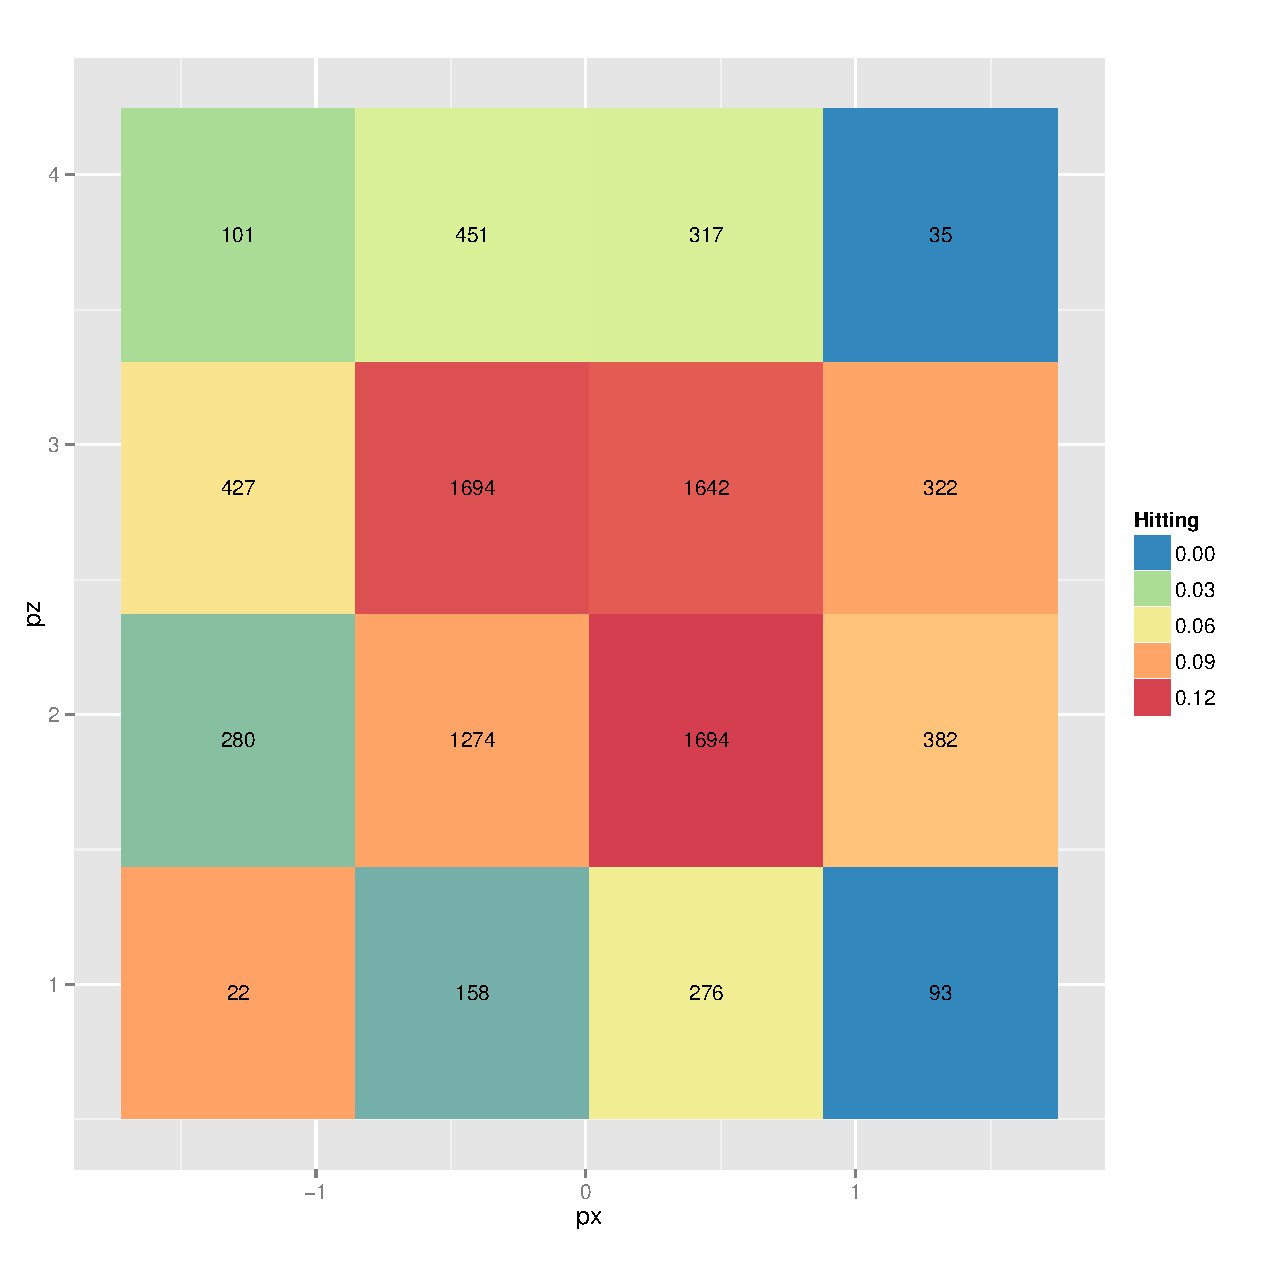
\includegraphics[scale=.2]{Images/Chapter4x4.pdf}
      	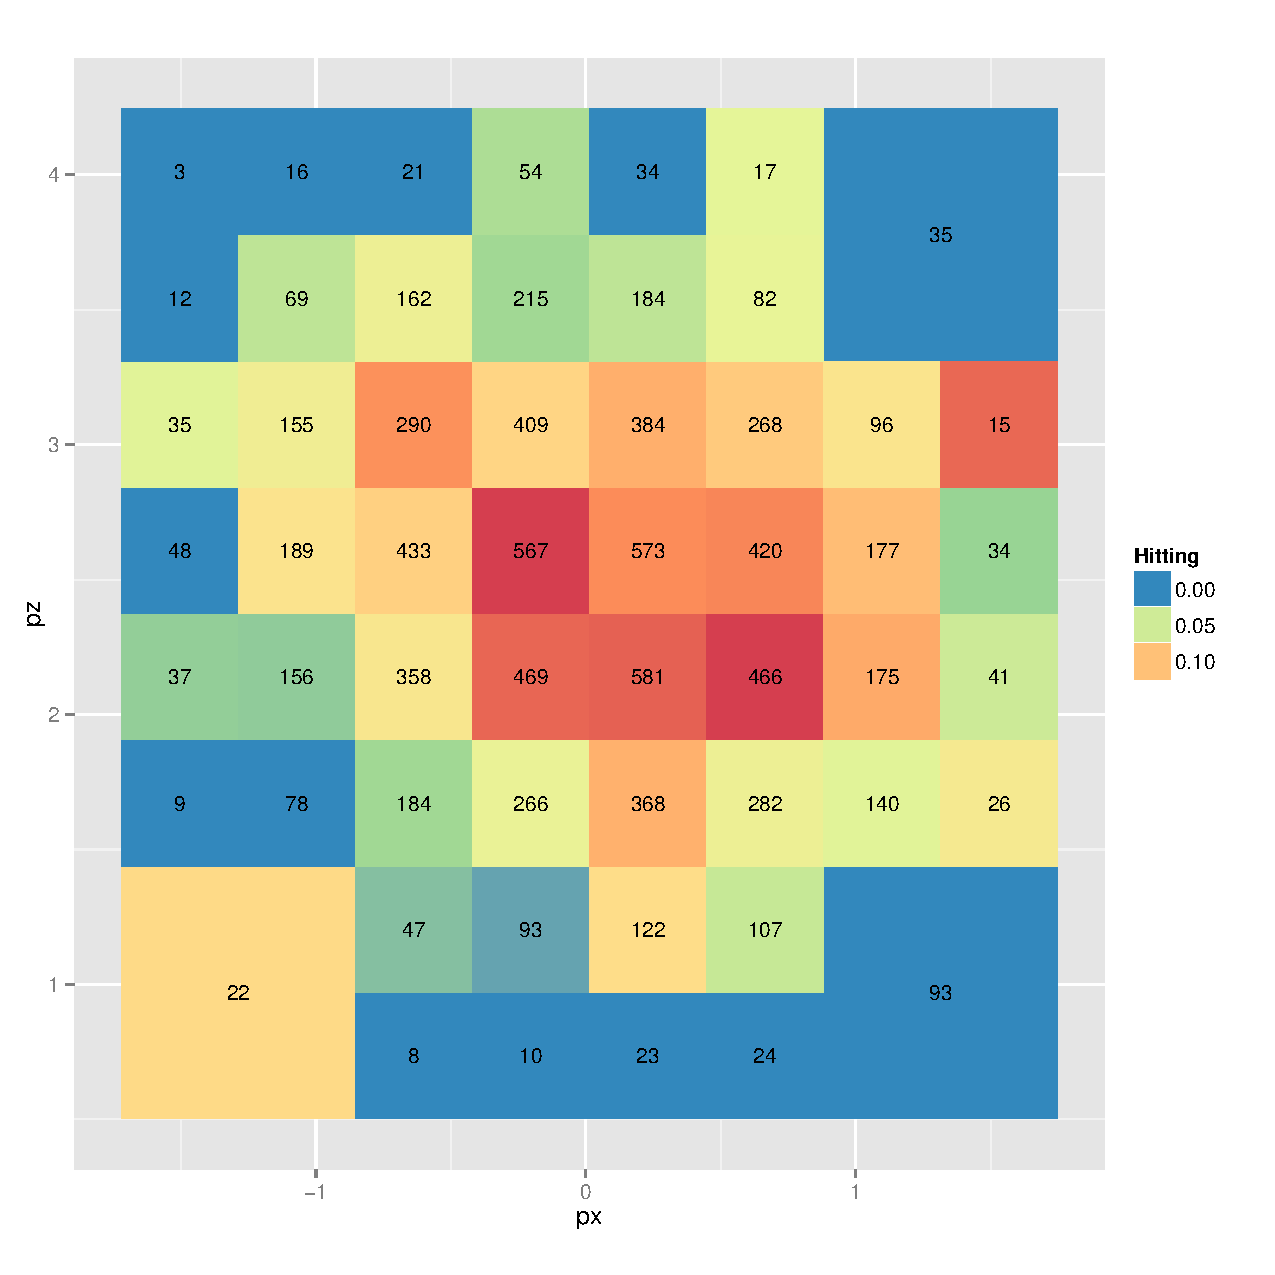
\includegraphics[scale=.2]{Images/Chapter8x8_100.pdf}
      	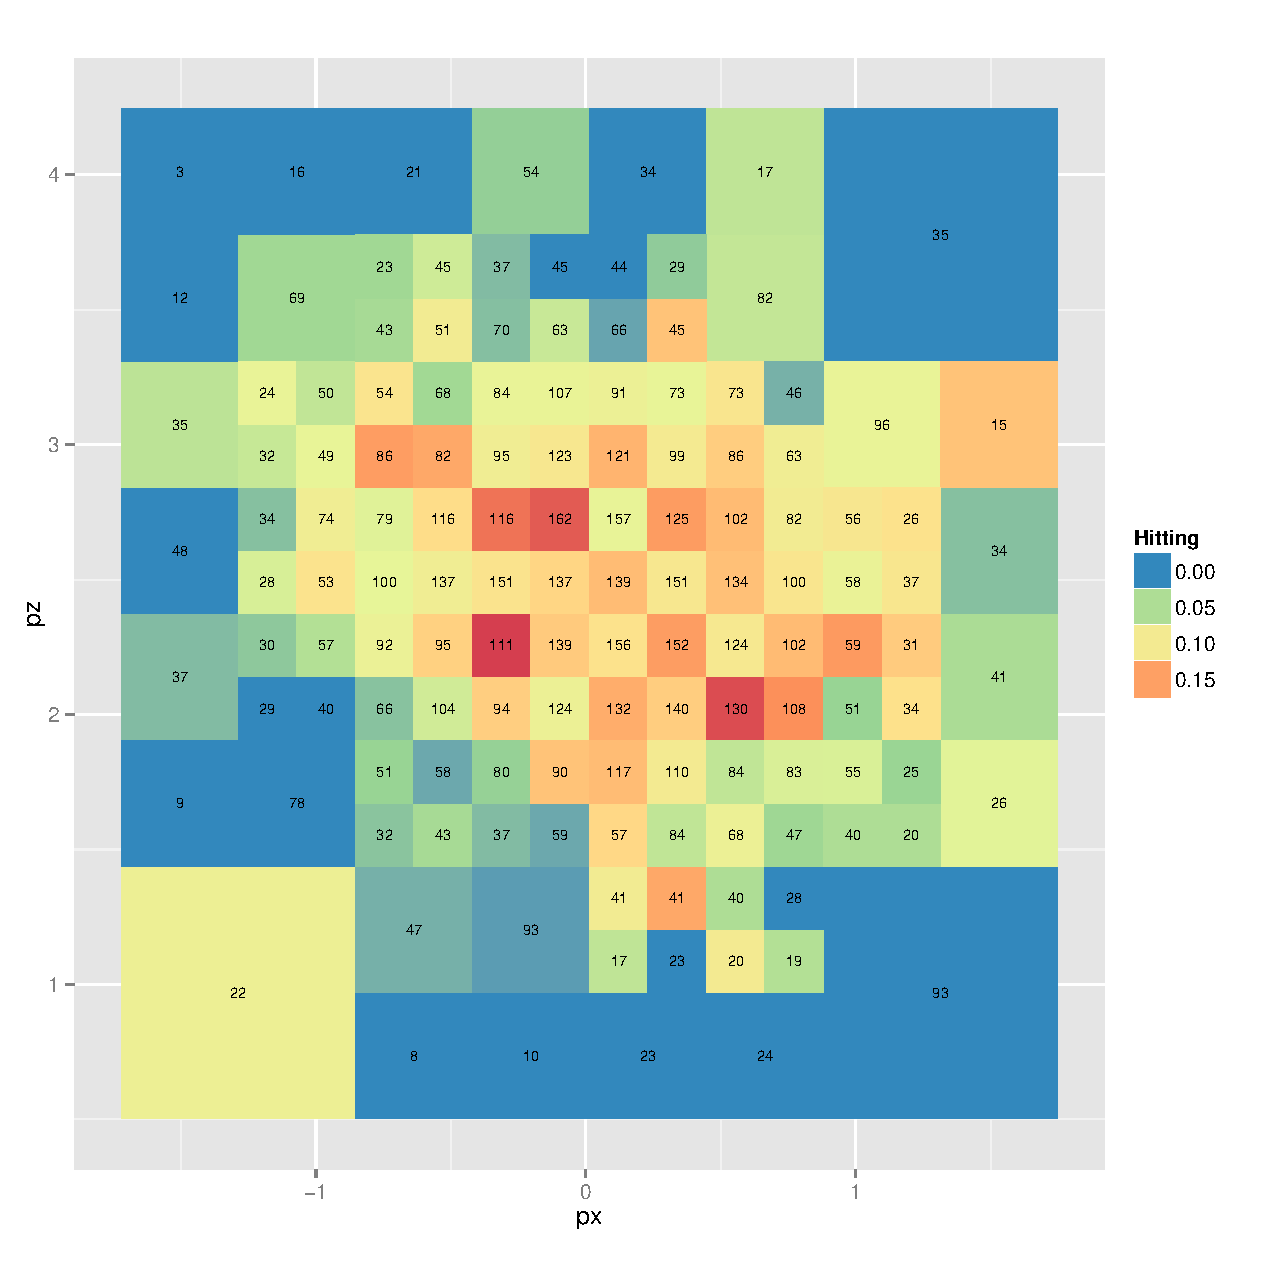
\includegraphics[scale=.2]{Images/Chapter16x16_100.pdf}
      	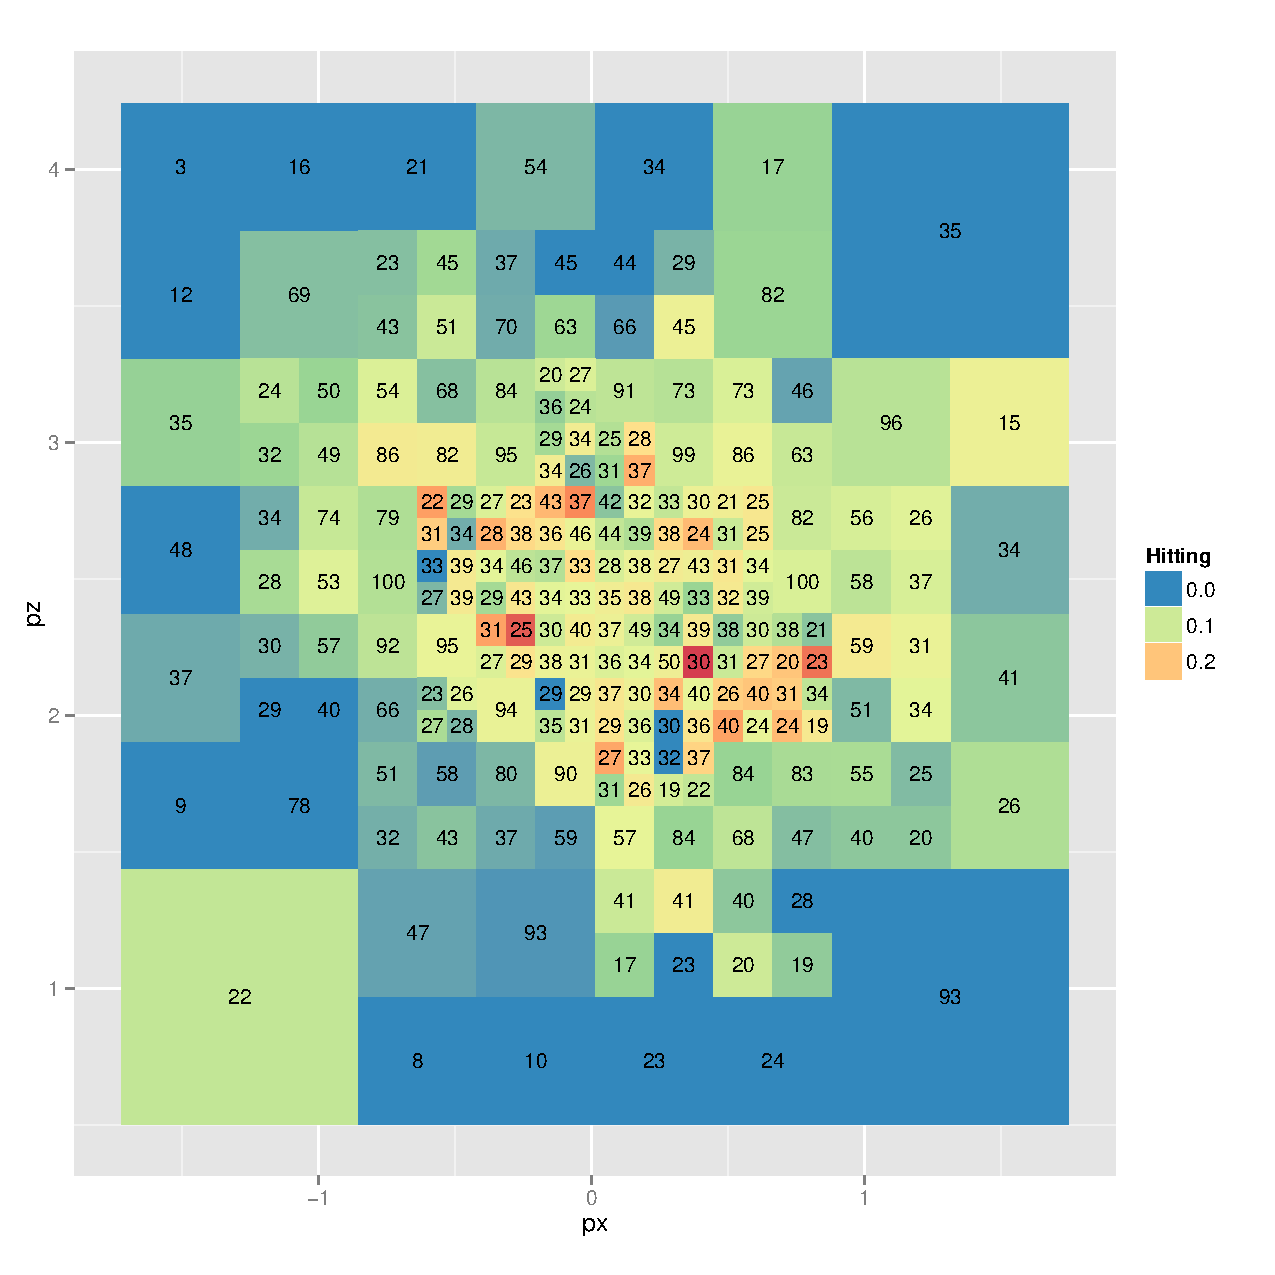
\includegraphics[scale=.2]{Images/Chapter32x32_100.pdf}
      	\caption{These heat maps convey the empirical batting average of batter 425509, Johnny Peralta, in each boxed region of the hitting zone. Each box maps $\hat{p}_{b}$ to a color. The number printed on each box represents the number of pitches the hitter swung at that passed through that box. All boxes with a sample size greater than 100 in each heat map have been subdivided in the subsequent heat map.}
\end{figure} 	
Compare this sequence for stopping rule $n_{b} < 100$, to Figure 1.8 for stopping rule $n_{b} < 200$. The the top row of maps in Figure 1.8 matches exactly the top row of maps in Figure 1.9. However, notice in the four by four heat map that $100 < n_{158} < 200, \text{ and } 100 < n_{101} < 200$. This implies diverging paths, where one stopping rule prevents further subdivision, while the other compels further subdivision.
        \begin{figure}[H]
      	\centering      
      	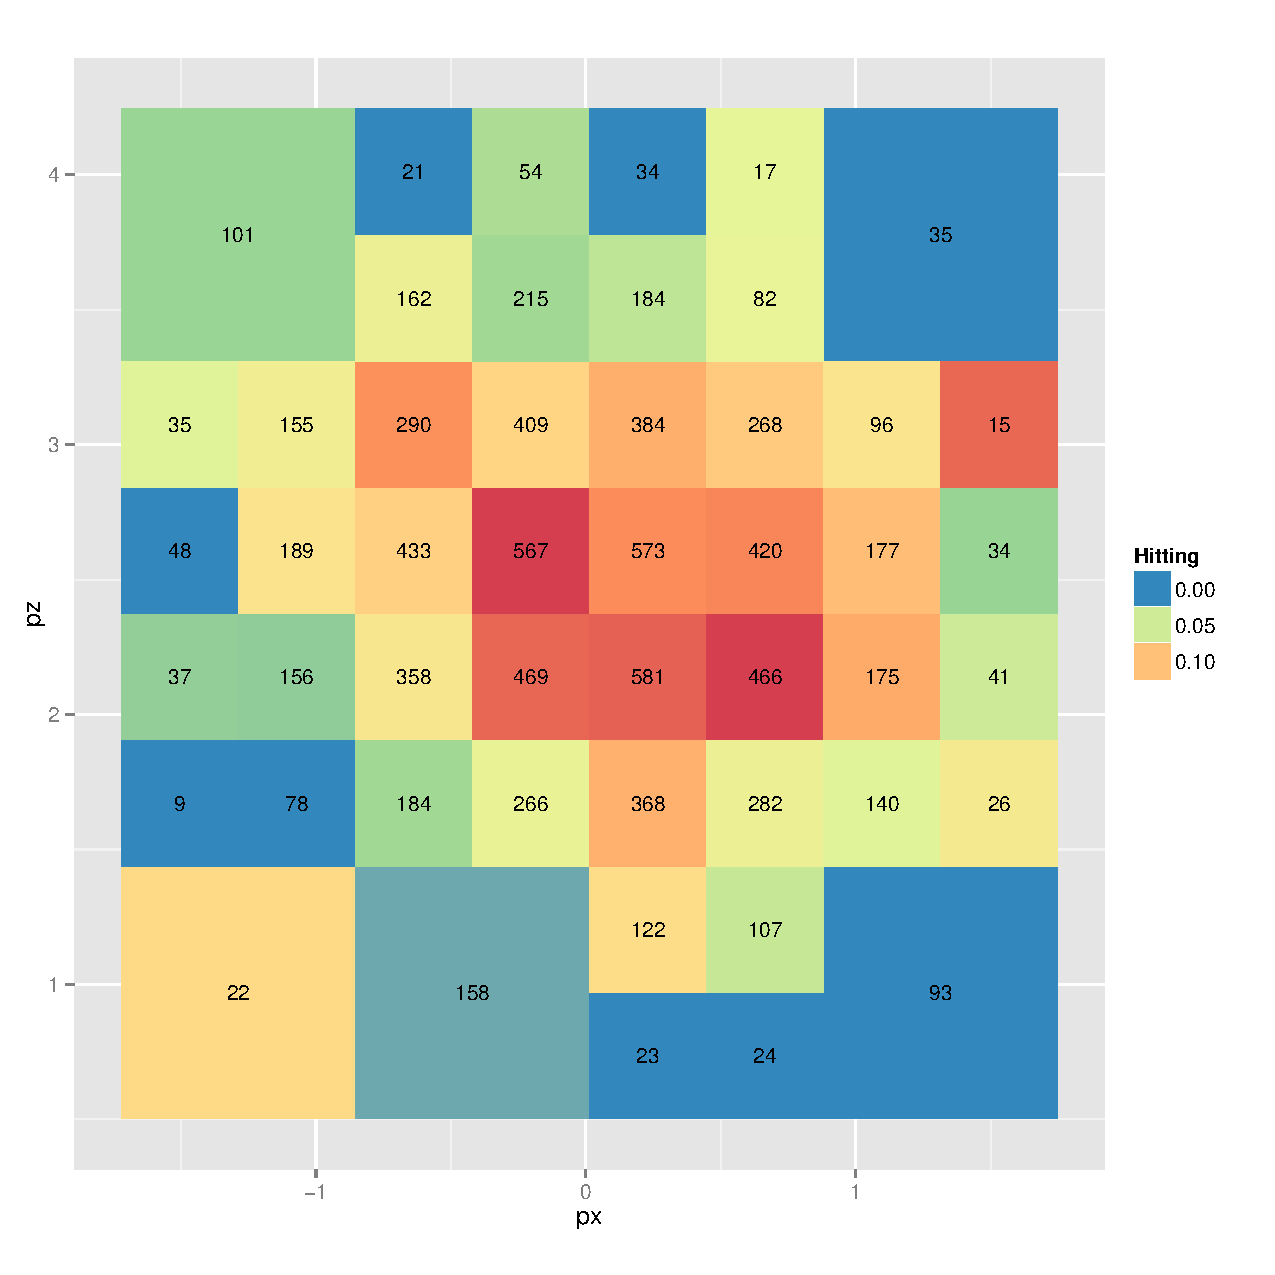
\includegraphics[scale=.25]{Images/Chapter8x8_200.pdf}
      	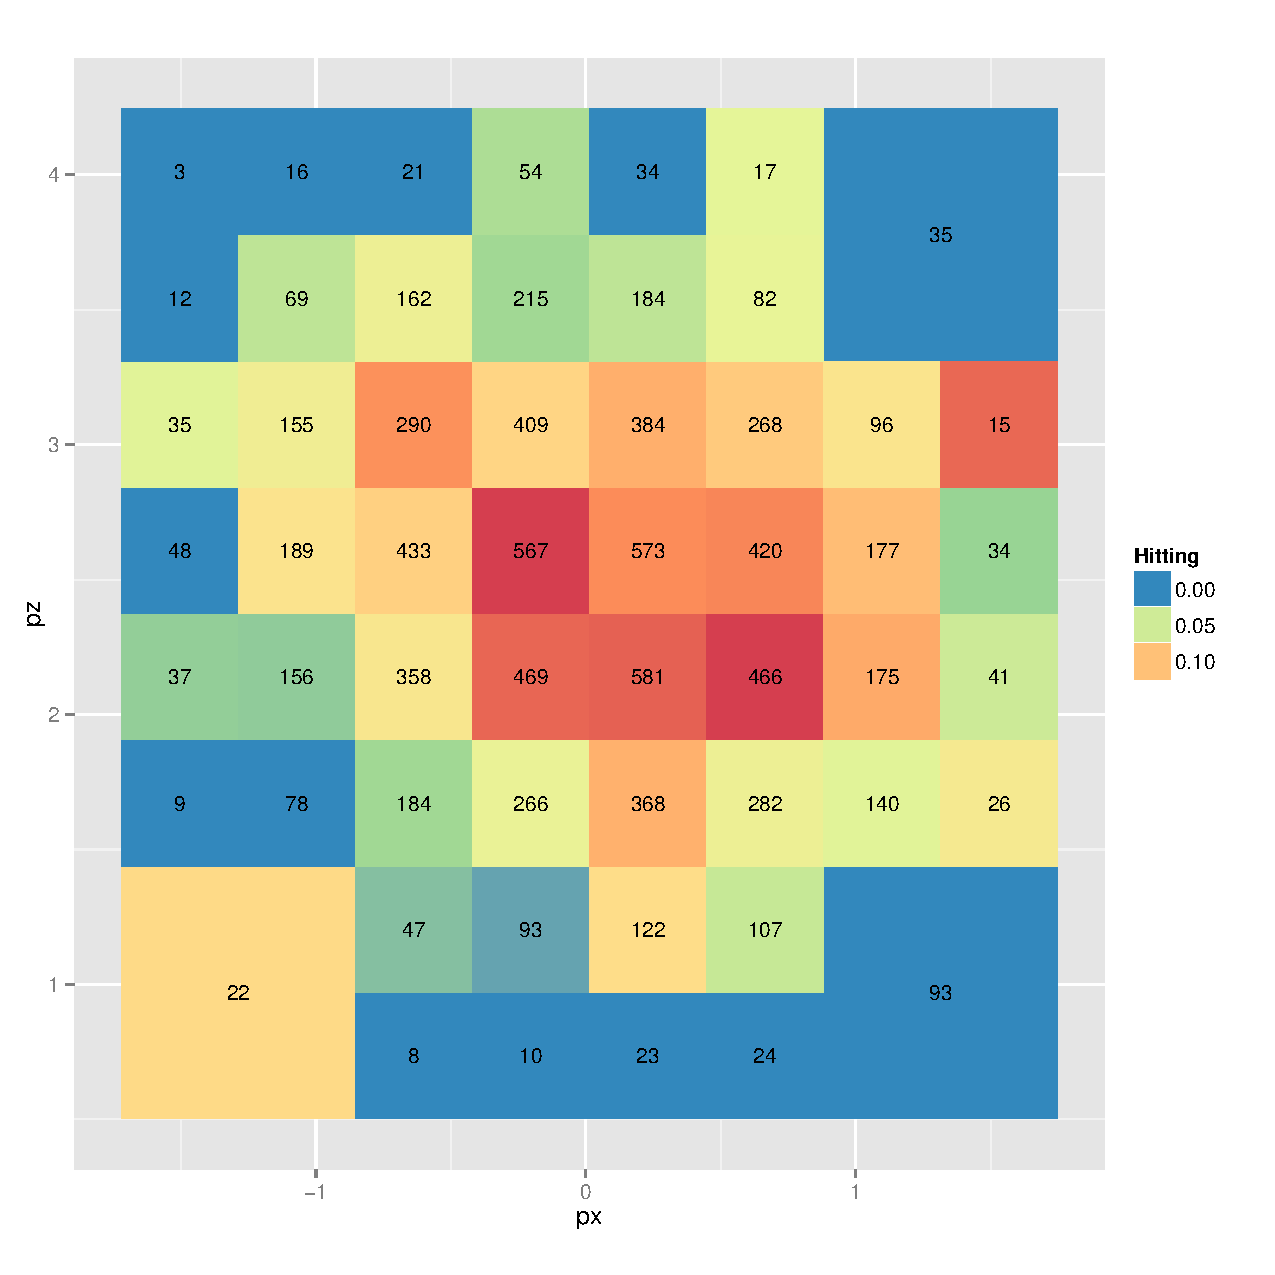
\includegraphics[scale=.25]{Images/Chapter8x8_100.pdf}
      	\caption{Variable-resolution heat maps diverge when box totals fall between sample size stopping rules. Boxes 158 and 101 remain for stopping rule $n_{b} < 200$ (left), but further subdivided for stopping rule $n_{b} < 100$ (right). Context should guide stopping rule selection}
\end{figure} 
We see the bottom left heat maps in Figures 1.8 and 1.9, shown in Figure 1.10, differ in the number of boxes of each size, and the total number of boxes. 

This differences increase at the next iteration, where the stopping rule $n_{b} < 100$ requires 28 box subdivisions, shown in Figure 1.9; and $n_{b} < 200$ gives 16 box subdivisions, shown in Figure 1.8.
        \begin{figure}[H]
      	\centering      
      	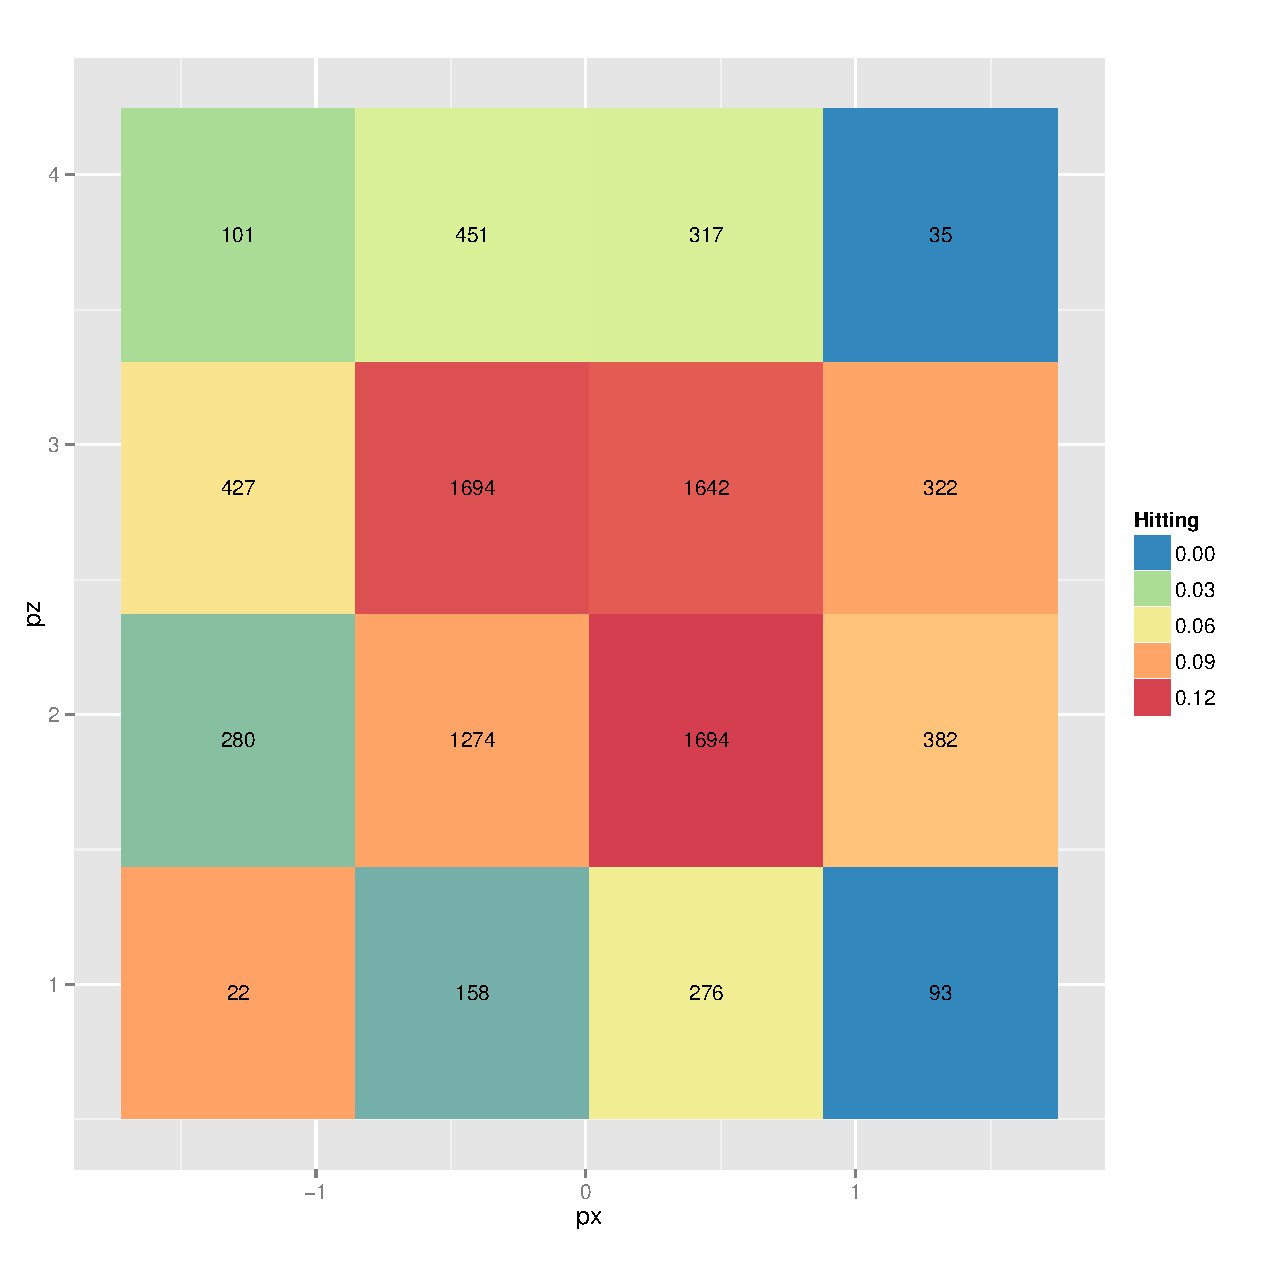
\includegraphics[scale=.2]{Images/Chapter4x4.pdf}
      	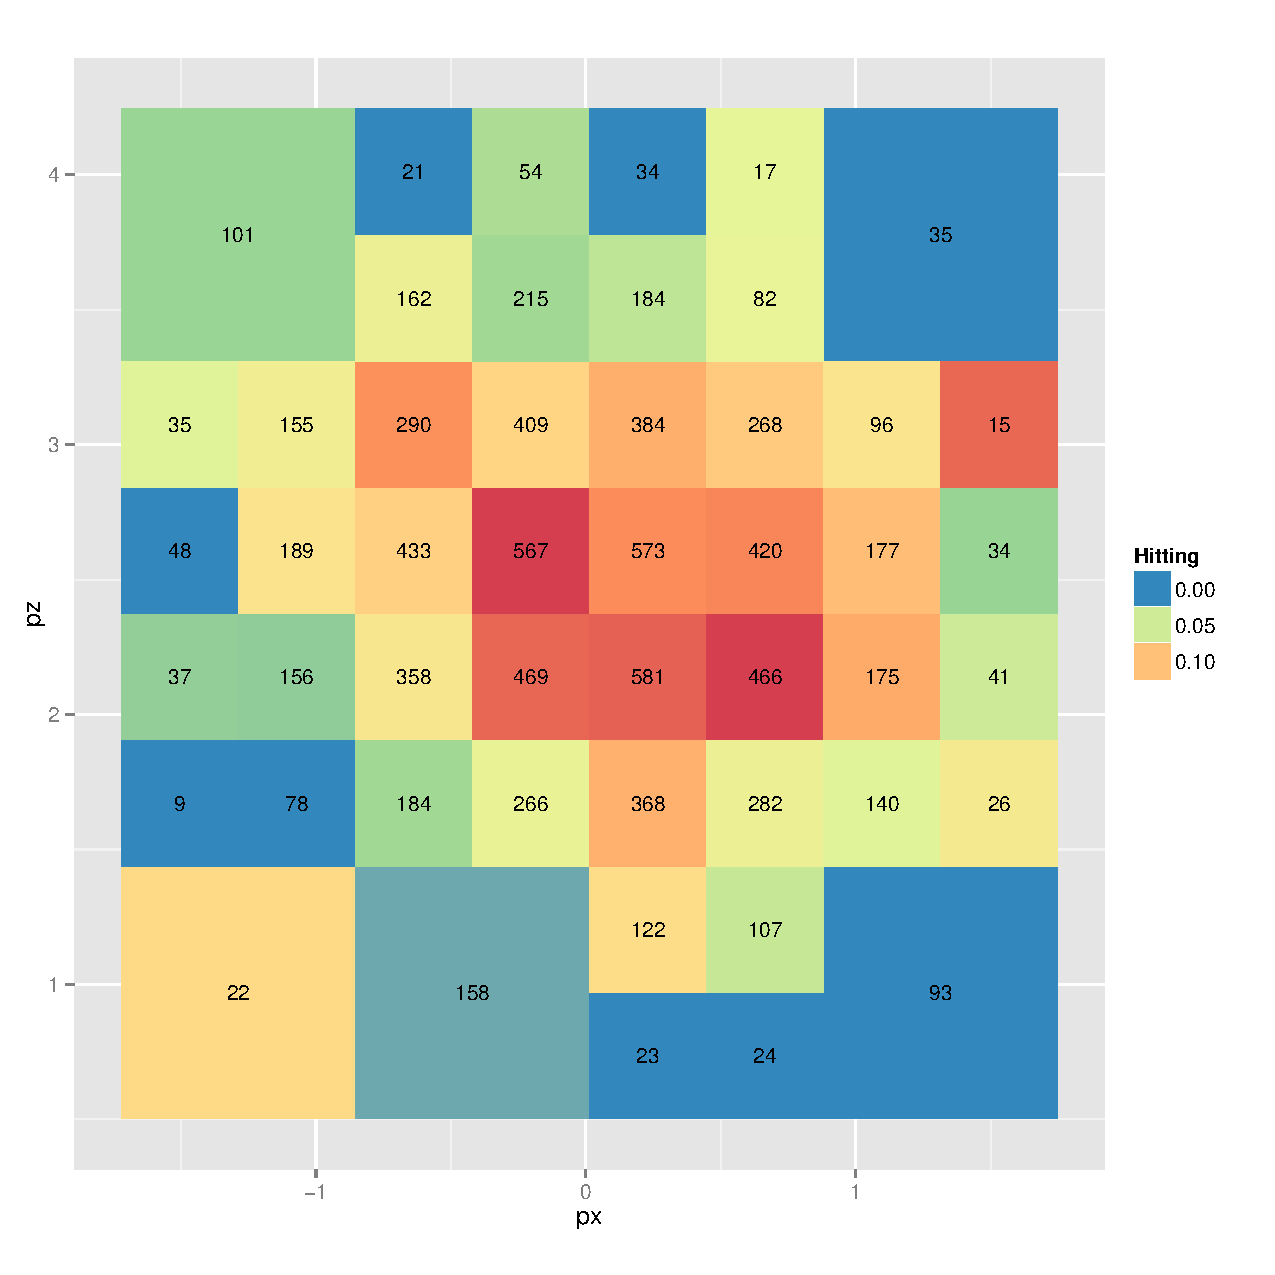
\includegraphics[scale=.2]{Images/Chapter8x8_200.pdf}
      	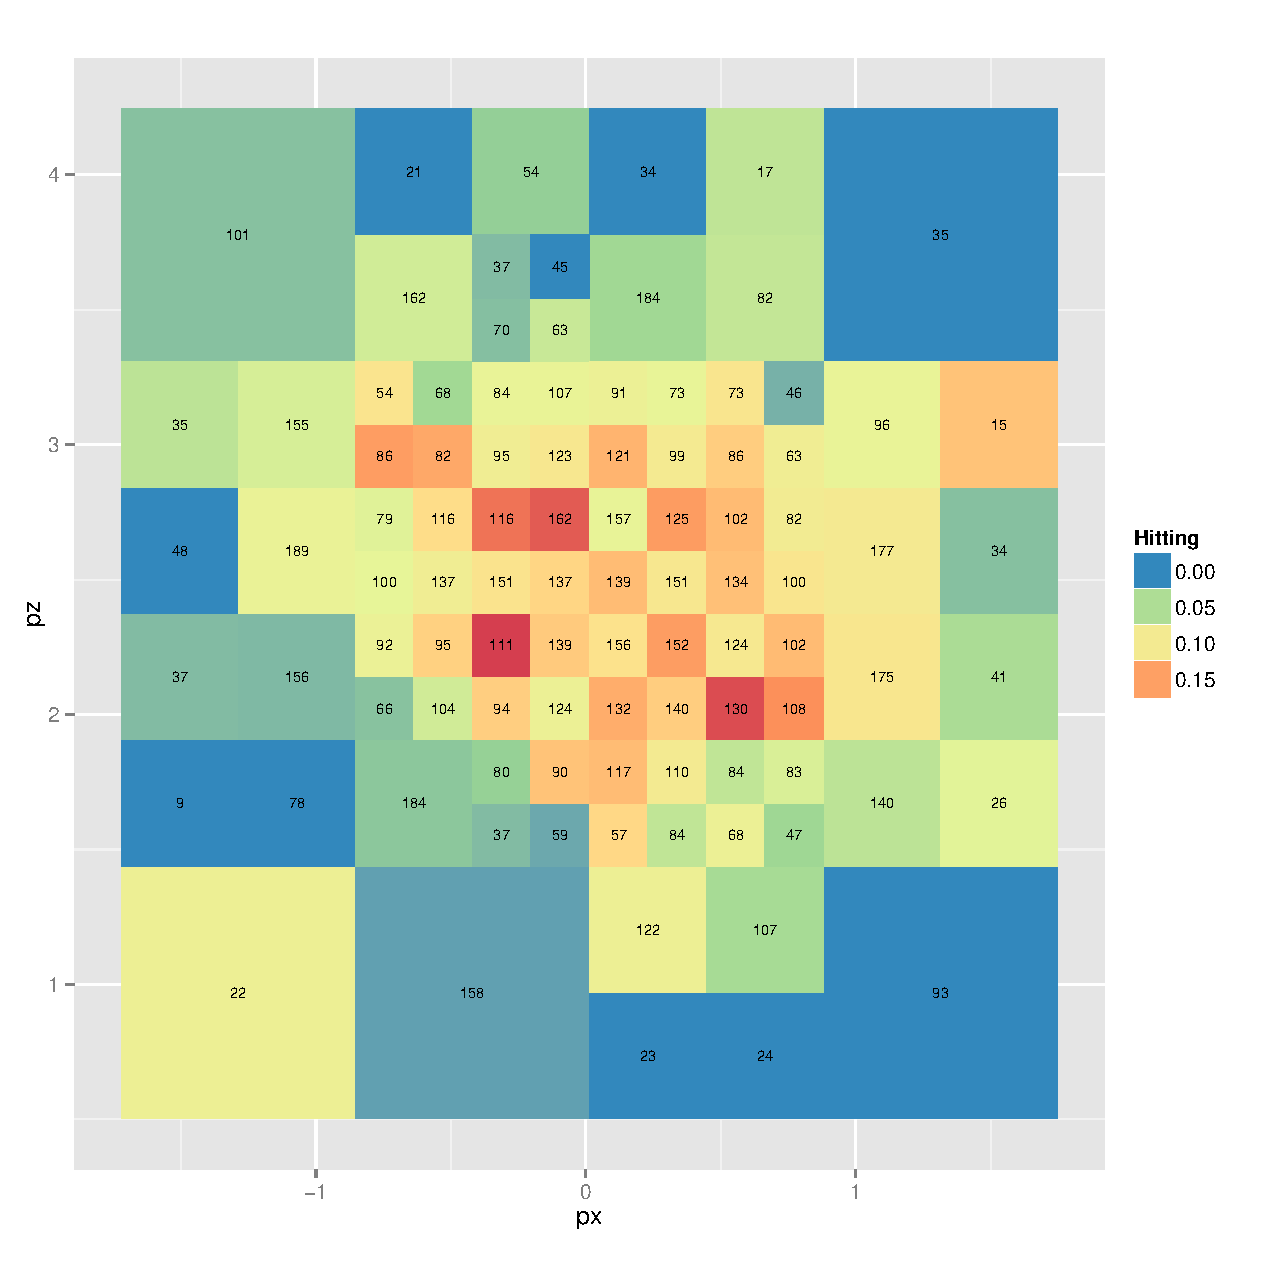
\includegraphics[scale=.2]{Images/Chapter16x16_200.pdf}
      	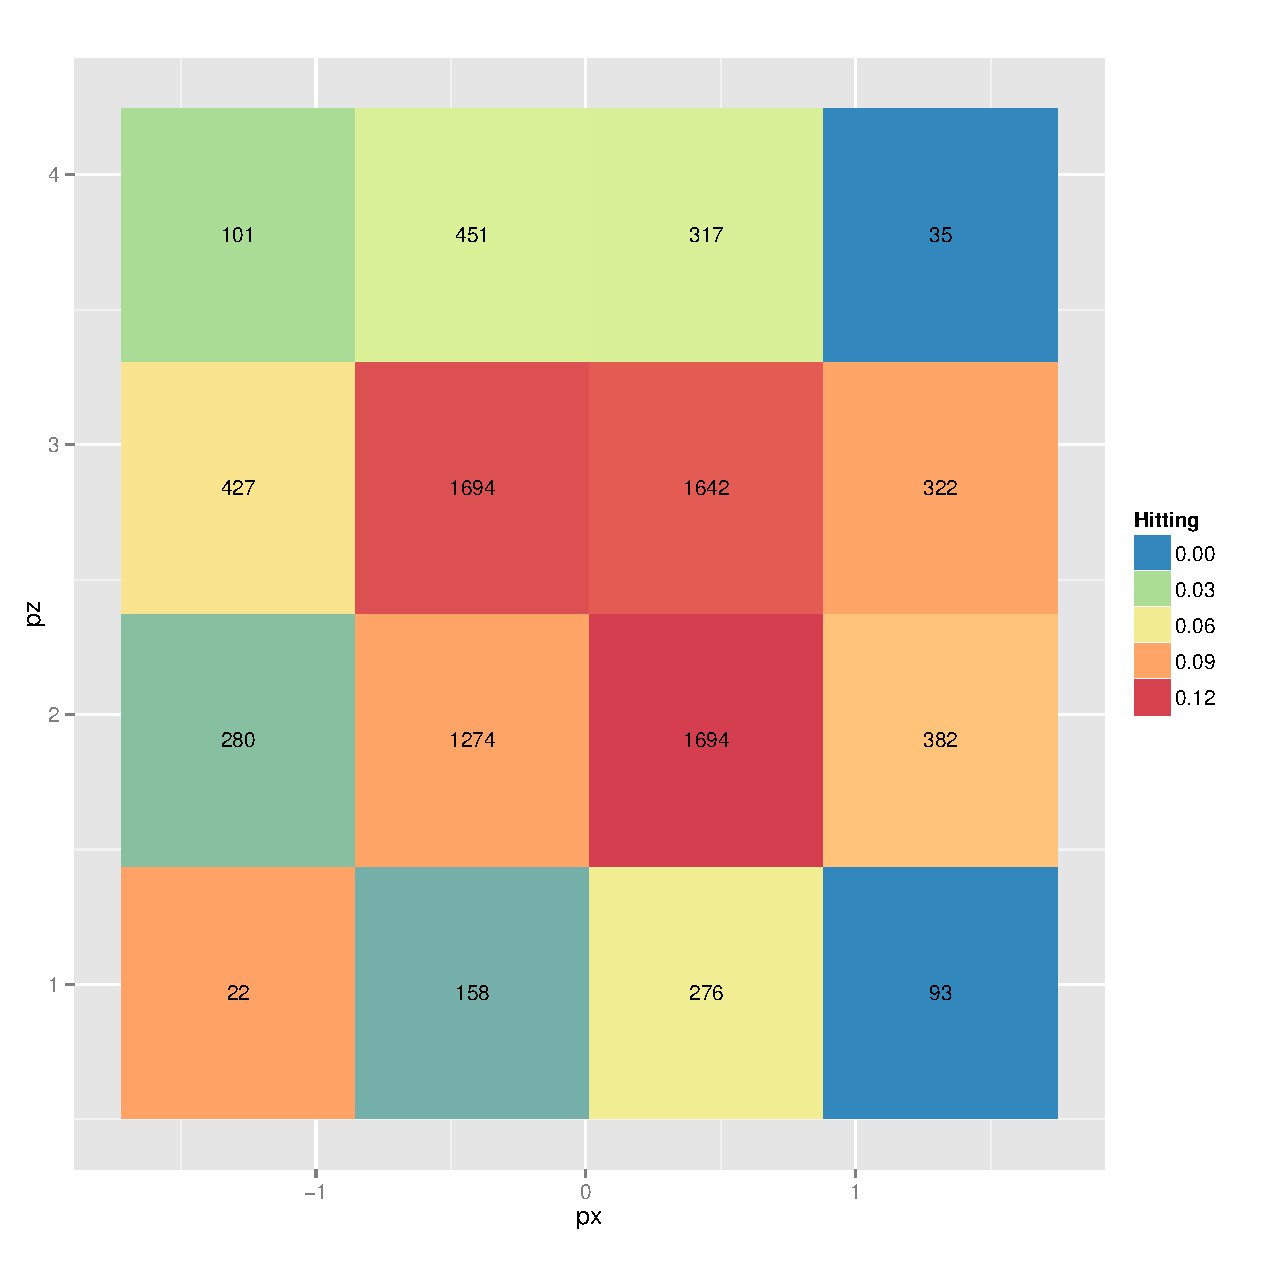
\includegraphics[scale=.2]{Images/Chapter4x4.pdf}
      	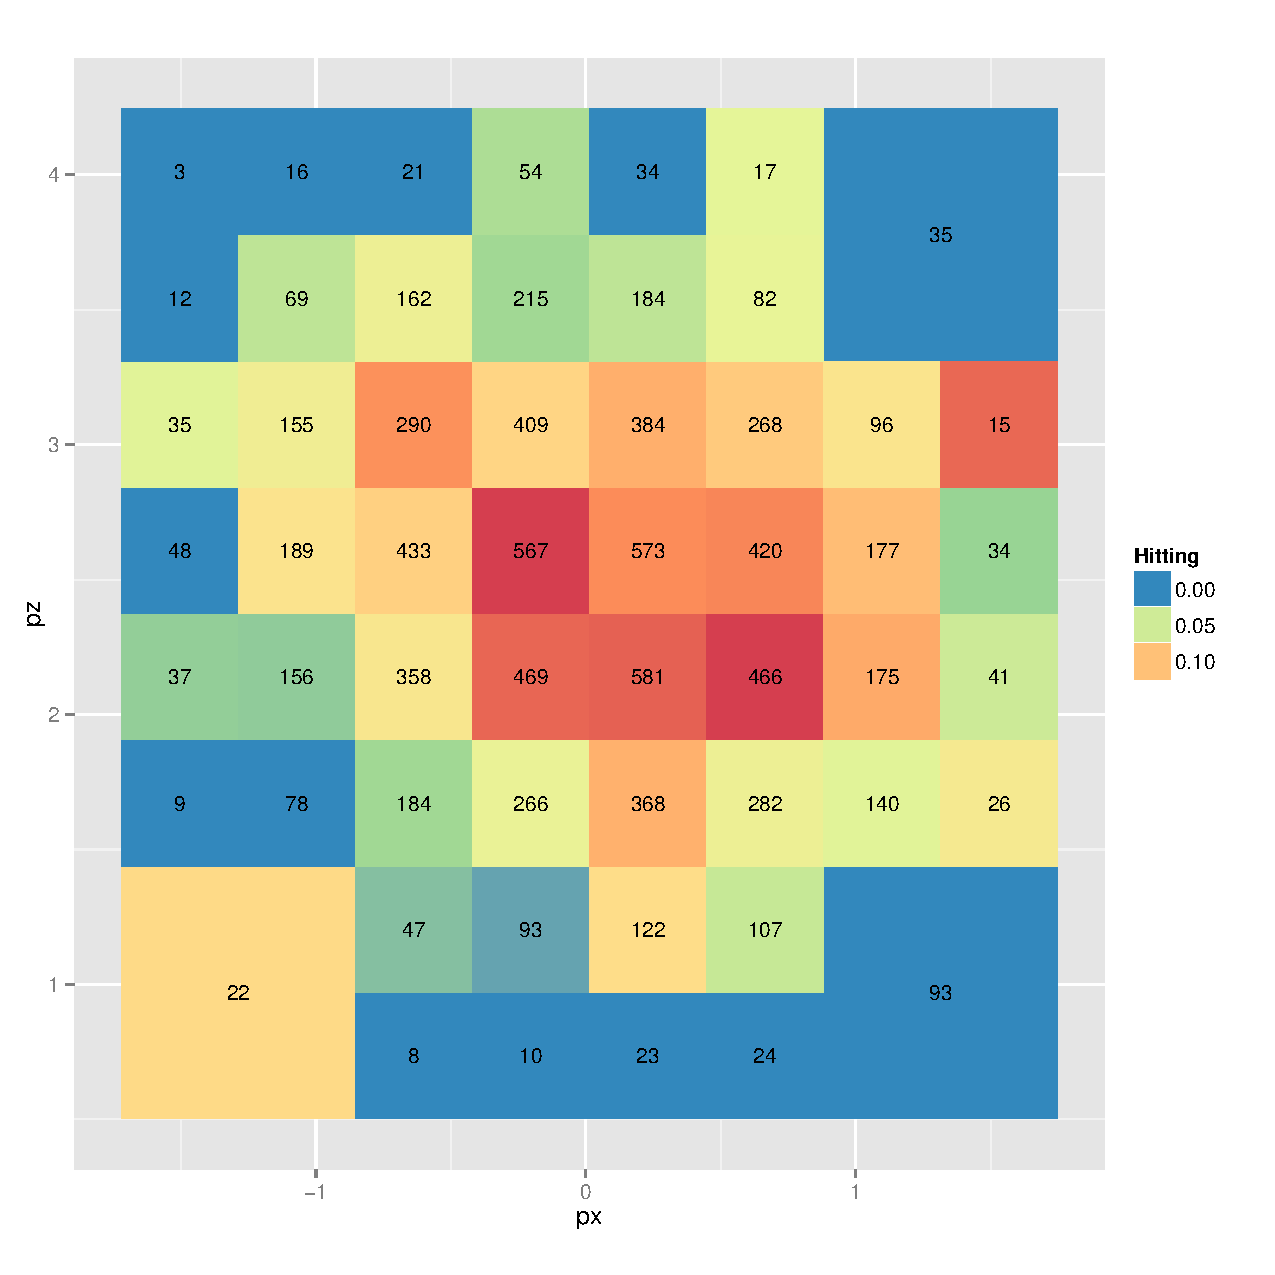
\includegraphics[scale=.2]{Images/Chapter8x8_100.pdf}
      	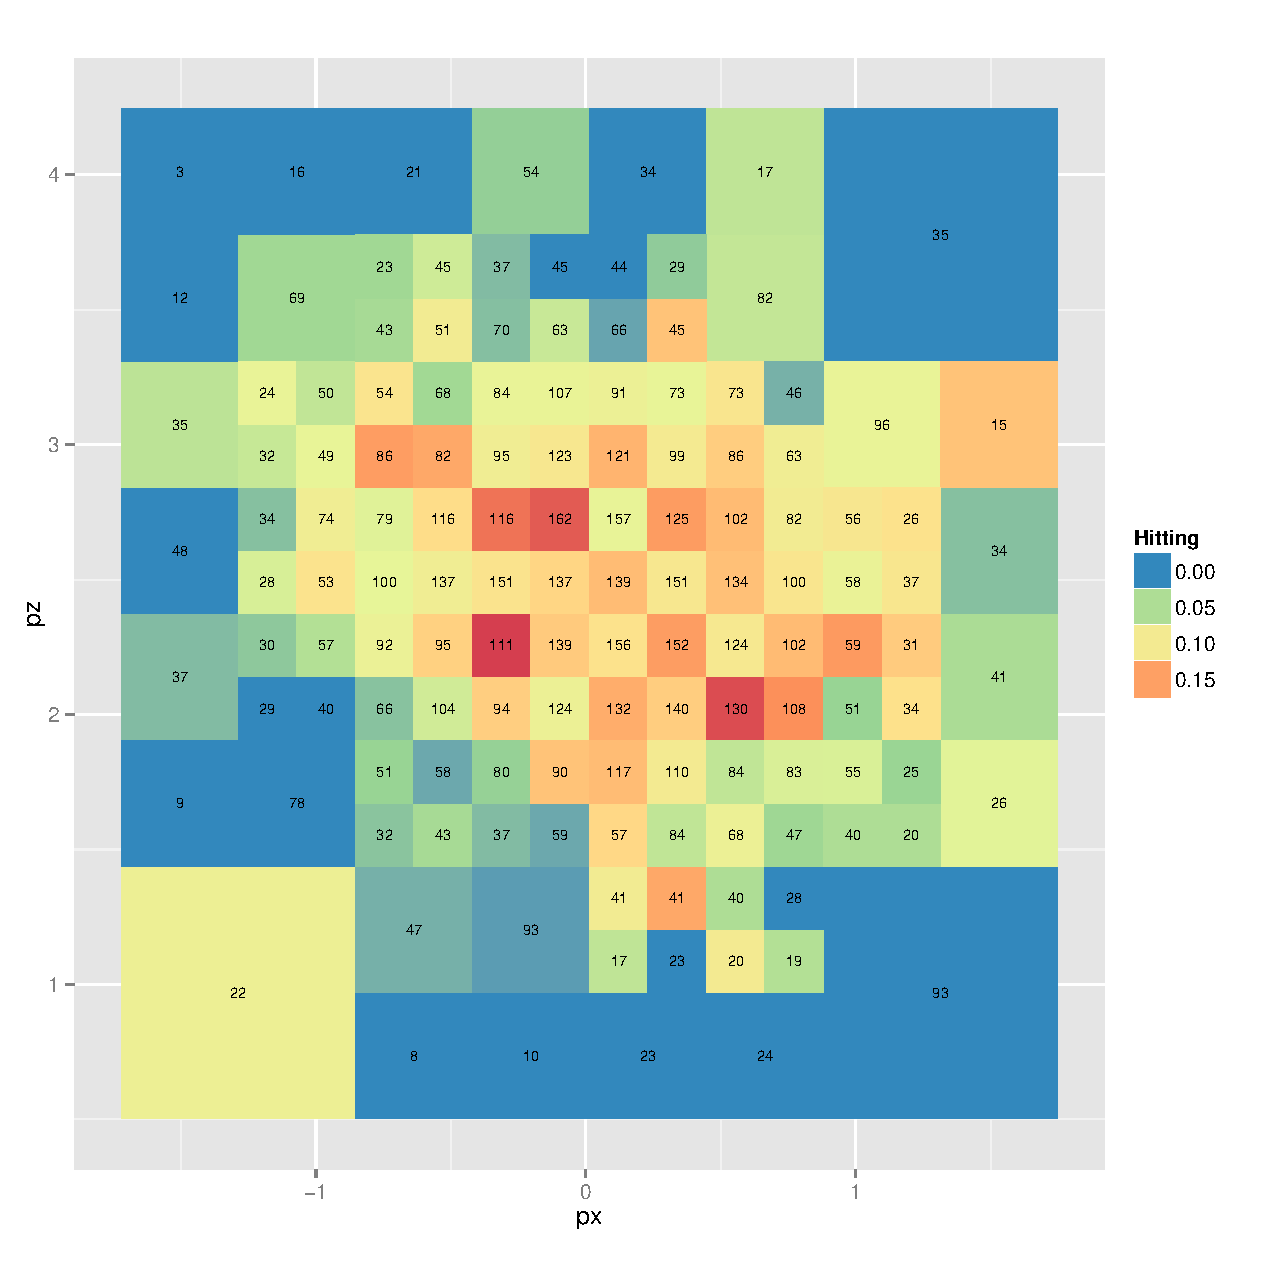
\includegraphics[scale=.2]{Images/Chapter16x16_100.pdf}
      	\caption{Variable-resolution heat maps diverge when box totals fall between sample size stopping rules. The top row of maps subdivides according to stopping rule $n_{b} < 200$; the bottom row further subdivides for stopping rule $n_{b} < 100$. The stopping rules concur through three iterations, the last of which we see first in each row. However, the next two iterations produce different maps. Context should guide stopping rule selection.}
\end{figure}

\subsection{Hitter vs. Pitcher} % ===================== =======
In this section, for illustrative purposes, we interpret features of the best--in this author's opinion--Johny Peralta variable-resolution heat map. Toward this end, we first describe basic strategy considerations in the hitter vs. pitcher matchup. 

\subsubsection{Context}
At the basic level, the pitcher wants to get outs and avoid baserunners; and hitters want to avoid outs and get on base. We are concerned with pitch location in this study, so we want to understand the pitch-swing location decisions; where the pitcher decides to throw, and which pitches the hitter decides to swing at. 

Three primary factors influence pitch-swing location: pitcher game theoretic strategy, pitch location margin of error (distance by which a pitch misses its intended target), and game state. Game theoretic strategy concerns the pitcher's knowledge of the hitter's strengths and weaknesses, and the hitter's reciprocal knowledge. Margin of error concerns the pitcher's tendency to miss his intended target by some amount. The game state includes the count (number of balls and strikes), the number of outs, and baserunner presence/absence. Two example game state pressures include the increased penalty for throwing a pitch outside the strike zone on a three ball count (the runner gets on base at four balls); and the increased penalty for a hit with a runner in ``scoring position.'' Our data includes pitches across all game states, so we will not rely on them for interpretation. Instead, we focus on game theory and margin of error rationale. 

\subsubsection{Interpretation}
Figure 1.13 gives, in the opinion of this author, the best heat map for Johny Peralta.
        \begin{figure}[H]
      	\centering      
      	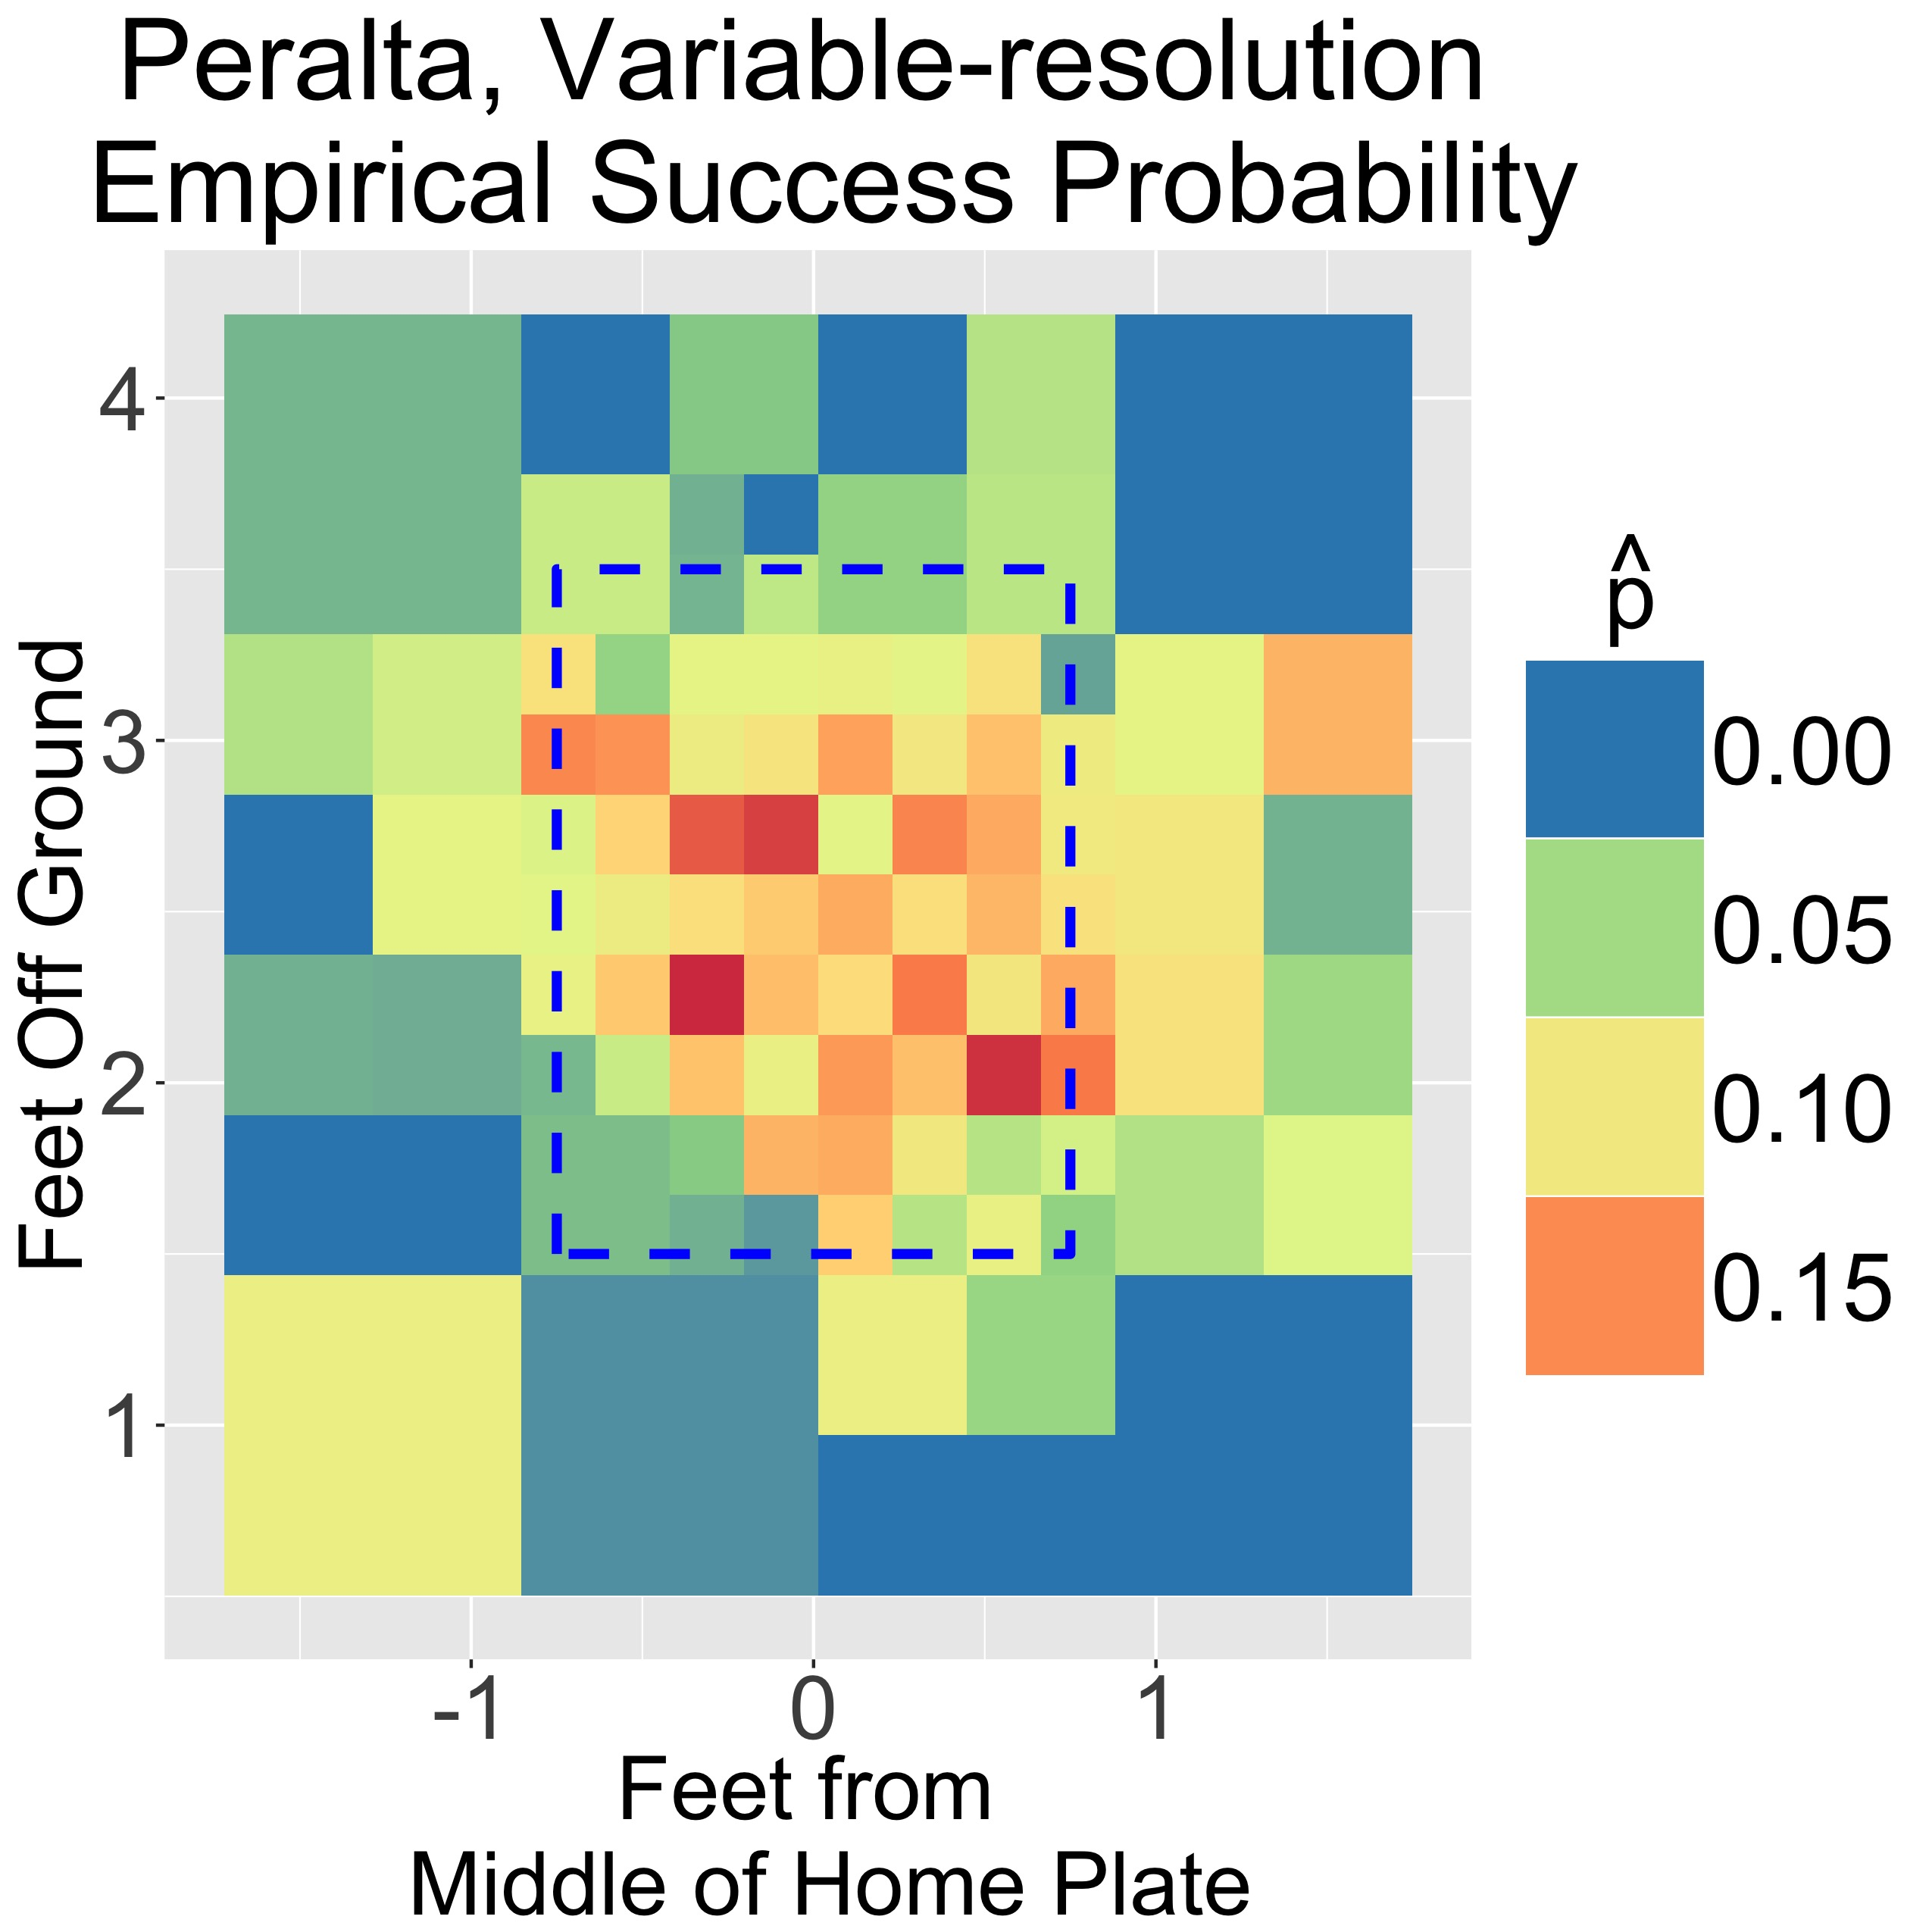
\includegraphics[scale=.1]{Images/Peralta_var-res.jpg}
      	\caption{This variable-resolution heat map for Johny Peralta gives spatial, empirical success probabilities; each box maps $\hat{b}_{b}$ to a color. In addition, the map conveys data density information; box size corresponds to the observation density, because subdivision persisted until box sample sizes dropped below 200.}
\end{figure}
The map gives spatial, empirical success probabilities for Johny Peralta. In regions of greater data density, and perhaps greater relevance, the map gives more spatially specific estimates. The size of the box conveys this density information, traditionally concealed in heat maps. This new feature derives from the fact that box subdivisions persist until box sample sizes drop below 200 (in this map).

Interpretable features abound. For example, Peralta generally saw and swing at far more pitches in the strike zone than out. Pitchers throw pitches in the strike zone because each strike is one step closer to an out, and each ball is one step closer to a baserunner. The same logic, with opposite goals/incentives, applies for the hitter. Therefore, many pitch-swings occur in the strike zone.

Notice the larger boxes in the lower left, upper left, and upper right of the strike zone. This implies Peralta saw and/or swung at fewer pitches in these locations. To explain, consider a pitch aimed for the bottom left of the strike zone. Missing the box below or to the left yields a ball, a result unambiguously in the hitter's favor; one step closer to the fourth ball of an at bat, when the rules award the hitter first base. In contrast, any swing, even those at the most hitter-favoring locations, yield an out with non-zero probability.

Elsewhere, boxes toward the middle of the strike zone contain more observations; finer resolution implies Peralta sees and/or swings at more pitches there. This region also seems to have greater success probabilities $\hat{p}_{b}$ (warmer colors), indicating Peralta indeed hits pitches in the center of the hitting zone better than pitches toward the edges of the hitting zone. In particular, the warmest boxes seem to be quite vertically centered. This indicates Peralta deals with horizontal variation better than vertical variation--an actionable insight! Peralta will swing at pitches in the middle of the strike zone almost every chance he gets.

Why then, would pitchers throw pitches there? Pitchers throw through the middle of the hitting zone more frequently for a few reasons. First, aiming for the midde of the strike yields the highest probability of a strike; missing the target by up to ten inches in any direction still yields a strike. Similarly, when aiming away from the middle of the strike zone some pitches miss their target and end up in the middle of the strike zone. 

Of the four strike zone corner locations, Peralta enjoyed the most success low and inside. The orange color of box 22, compares favorably to the otherwise green, yellow, and blue low or inside pitches. Therefore, we speculate that pitchers simply avoided this location when pitching low or inside. On the other hand, Peralta enjoyed as much or more success in middle of the strike zone, boxes 1694, 1642, 1274, and 1694; and saw and swung at far more pitches there. Why did pitchers not avoid those locations too? They probably tried! However, game state pressures frequently compel pitchers to throw a strike, and the middle of the strike zone offers the pitcher his best chance; missing the target in the middle of the strike zone will, more often than any other location, still result in a strike. In addition, Peralta, like almost all hitters, strives to swing almost every time the pitcher accidentally throws the easiest pitch to hit.

He probably swings at these pitches less often because they are, quite simply, difficult to hit successfully. On the other hand, pitchers may {\it throw} to these spots less often because of their relatively greater associated risk; they are less likely to induce swings, and small errors yield an unfavorable outcome. We delve into these baseball strategic nuances later.

% *Alix: ``I wonder if there's any literature on the physics from a hitter's perspective in terms of how small a difference in location is even detectable.

% \subsection{Appendix: VarResHM, An R Package}

% 
% \bibliography{Baseball}
% 
% \end{document}